\section{分子结构基础 · 超级充实版}\label{ux5206ux5b50ux7ed3ux6784ux57faux7840-ux8d85ux7ea7ux5145ux5b9eux7248}

\begin{center}\rule{0.5\linewidth}{0.5pt}\end{center}

\subsection{学习目标}\label{ux5b66ux4e60ux76eeux6807}

\begin{itemize}
\tightlist
\item
  能区分三大化学键类型(离子键/共价键/金属键)，用电负性差判断键型
\item
  理解共价键的\西格马/\派本质，识别\西格马键和\派键，判断配位键中的\西格马-给予/\派-反馈
\item
  能画出常见分子/离子的 Lewis 结构，计算形式电荷并选择最优共振式
\item
  能用 AXₙEₘ 模型(VSEPR 理论)预测分子几何构型，处理孤对电子的位置选择
\item
  能根据分子形状和键角判断中心原子的杂化类型(sp/sp\textsuperscript{2}/sp\textsuperscript{3}/sp\textsuperscript{3}d/sp\textsuperscript{3}d\textsuperscript{2})
\item
  能判断离域\派键的形成条件并写出 \派ₙᵐ 表示
\item
  能用等电子体原理推断未知分子/离子的结构
\item
  能画出第二周期双原子分子的 MO 能级图，计算键级并判断磁性
\item
  能区分分子间力类型，用氢键解释反常物性
\end{itemize}

\begin{center}\rule{0.5\linewidth}{0.5pt}\end{center}

\subsection{一、化学键基础 --- 原子为什么成键？键有哪些类型？}\label{ux4e00ux5316ux5b66ux952eux57faux7840-ux539fux5b50ux4e3aux4ec0ux4e48ux6210ux952eux952eux6709ux54eaux4e9bux7c7bux578b}

在学习如何画分子结构之前，我们需要先回答两个根本问题：\textbf{原子为什么要成键？} 以及 \textbf{键有哪些类型、怎么区分？} 这是理解后续所有内容的概念基础。

\textbf{教学洞察}：质心和周坤两套教学逻辑都以''成键本质\箭键型分类\箭电负性判据``作为分子结构的开篇。质心教学逻辑明确指出：''成键的本质是轨道重叠使系统能量降低''，周坤则强调电负性是''从原子结构到分子结构的桥梁概念''。\textbf{先把''为什么''和''是什么''搞清楚，再学''怎么画''。}

\subsubsection{1.1 为什么原子要成键？}\label{ux4e3aux4ec0ux4e48ux539fux5b50ux8981ux6210ux952e}

原子成键的根本驱动力是\textbf{降低系统能量}。孤立原子的电子处于高能态，当成键后电子在更广阔的空间中运动，动能降低，系统趋于稳定。

\textbf{核心原则}：成键 = 系统能量降低 \箭 稳定化。这就是为什么自然界中绝大多数原子不以单原子形式存在。

\subsubsection{1.2 三大基本键型}\label{ux4e09ux5927ux57faux672cux952eux578b}

化学键按成键方式分为三类，它们之间并非截然分开，而是存在连续过渡：

{\def\LTcaptype{none} % do not increment counter
\begin{longtable}[]{@{}
  >{\raggedright\arraybackslash}p{(\linewidth - 6\tabcolsep) * \real{0.2500}}
  >{\raggedright\arraybackslash}p{(\linewidth - 6\tabcolsep) * \real{0.2500}}
  >{\raggedright\arraybackslash}p{(\linewidth - 6\tabcolsep) * \real{0.2500}}
  >{\raggedright\arraybackslash}p{(\linewidth - 6\tabcolsep) * \real{0.2500}}@{}}
\toprule\noalign{}
\begin{minipage}[b]{\linewidth}\raggedright
键型
\end{minipage} & \begin{minipage}[b]{\linewidth}\raggedright
本质
\end{minipage} & \begin{minipage}[b]{\linewidth}\raggedright
特征
\end{minipage} & \begin{minipage}[b]{\linewidth}\raggedright
典型实例
\end{minipage} \\
\midrule\noalign{}
\endhead
\bottomrule\noalign{}
\endlastfoot
\textbf{离子键} & 正负离子间的静电引力 & 无方向性、无饱和性 & NaCl、CsCl \\
\textbf{共价键} & 原子间共用电子对 & 有方向性、有饱和性 & H\textsubscript{2}、H\textsubscript{2}O、CO\textsubscript{2} \\
\textbf{金属键} & 金属阳离子与自由电子的相互作用 & 无方向性、无饱和性 & Fe、Cu、Na \\
\end{longtable}
}

\begin{figure}[H]\centering
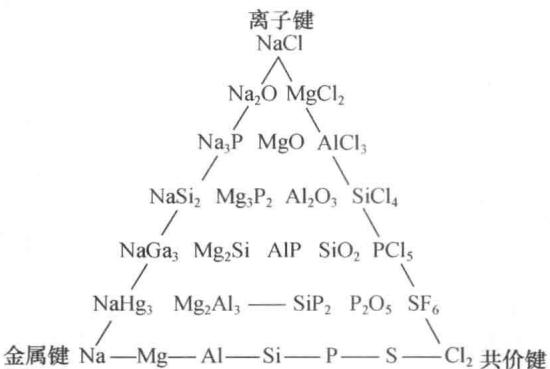
\includegraphics[width=0.45\textwidth,keepaspectratio]{media/13-6-bond-type-transition-triangle-ionic-covalent-metallic.jpg}
\caption{化学键类型连续谱—离子键、共价键、金属键之间存在渐变过渡关系}
\end{figure}

\textbf{离子键要点}：
- 由电负性差大的原子间形成(通常 Δχ \textgreater{} 1.9)
- 特点：无方向性(静电场各向同性)、无饱和性(每个离子可吸引周围所有异号离子)
- 离子极化效应(Fajans 规则)：当正离子电荷高、半径小，负离子电荷高、半径大时，离子键向共价键过渡

\begin{figure}[H]\centering
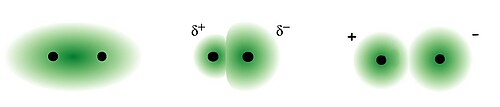
\includegraphics[width=0.45\textwidth,keepaspectratio]{media/covalent-ionic-bonds-wikipedia.jpg}
\caption{共价键(左：非极性共价；中：极性共价 $\delta$···$\delta$；右：离子键 + −)}
\end{figure}

{\def\LTcaptype{none} % do not increment counter
\begin{longtable}[]{@{}
  >{\raggedright\arraybackslash}p{(\linewidth - 4\tabcolsep) * \real{0.3333}}
  >{\raggedright\arraybackslash}p{(\linewidth - 4\tabcolsep) * \real{0.3333}}
  >{\raggedright\arraybackslash}p{(\linewidth - 4\tabcolsep) * \real{0.3333}}@{}}
\toprule\noalign{}
\begin{minipage}[b]{\linewidth}\raggedright
极化因素
\end{minipage} & \begin{minipage}[b]{\linewidth}\raggedright
促进极化(\箭共价性\上箭)
\end{minipage} & \begin{minipage}[b]{\linewidth}\raggedright
抑制极化(\箭离子性\上箭)
\end{minipage} \\
\midrule\noalign{}
\endhead
\bottomrule\noalign{}
\endlastfoot
正离子 & 电荷高、半径小(如 Al\textsuperscript{3+}) & 电荷低、半径大(如 Cs\textsuperscript{+}) \\
负离子 & 电荷高、半径大(如 I\textsuperscript{-}) & 电荷低、半径小(如 F\textsuperscript{-}) \\
电子构型 & 18e\textsuperscript{-} 或 18+2e\textsuperscript{-}(如 Ag\textsuperscript{+}、Pb\textsuperscript{2+}) & 8e\textsuperscript{-}(如 Na\textsuperscript{+}、Ca\textsuperscript{2+}) \\
\end{longtable}
}

\textbf{口诀}：``正离子小而正，负离子大而负，电子构型不规则---极化强，共价多。''

\textbf{金属键要点}：
- ``电子海''模型：金属原子失去部分价电子形成阳离子，自由电子在整个金属晶格中离域
- 解释金属特性：导电性(自由电子迁移)、导热性、延展性(离子层滑动不破坏键)

\subsubsection{1.3 电负性 --- 判断键型的标尺}\label{ux7535ux8d1fux6027-ux5224ux65adux952eux578bux7684ux6807ux5c3a}

\textbf{电负性}(Pauling 标度)衡量原子在分子中吸引共用电子对的能力，以 F = 4.0 为基准。

\begin{figure}[H]\centering
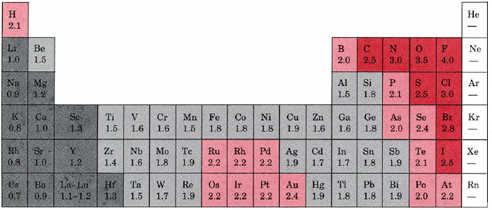
\includegraphics[width=0.45\textwidth,keepaspectratio]{media/11-25-electronegativity-periodic-trend.jpg}
\caption{电负性的周期表递变趋势}
\end{figure}

\begin{figure}[H]\centering
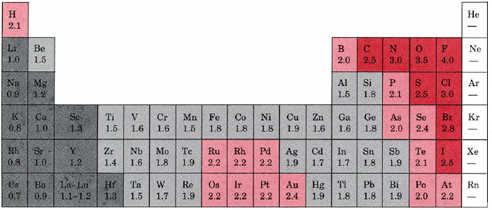
\includegraphics[width=0.45\textwidth,keepaspectratio]{media/electronegativity_table.jpg}
\caption{常见元素电负性(Pauling 标度)}
\end{figure}

\textbf{电负性周期趋势}：
- \textbf{同周期}从左到右递增(有效核电荷增大，原子半径减小)
- \textbf{同主族}从上到下递减(电子层数增多，屏蔽效应增强)

\textbf{Δχ 与键型判断}(经验阈值)：

{\def\LTcaptype{none} % do not increment counter
\begin{longtable}[]{@{}cll@{}}
\toprule\noalign{}
电负性差 Δχ & 键型 & 示例 \\
\midrule\noalign{}
\endhead
\bottomrule\noalign{}
\endlastfoot
\textless{} 0.4 & 非极性共价键 & H\textsubscript{2} (0), Cl\textsubscript{2} (0) \\
0.4 \textasciitilde{} 1.9 & 极性共价键 & HCl (0.9), H\textsubscript{2}O (1.4) \\
\textgreater{} 1.9 & 离子键 & NaCl (2.1), CsF (3.3) \\
\end{longtable}
}

\textbf{易错提醒}：Δχ = 1.9 的 HF 是\textbf{共价键}而非离子键---这是阈值的''灰区''。实际化学键是连续谱，Δχ 判据只是粗略指南。判断键型时还需结合 Fajans 规则(离子极化效应)综合判断。

\subsubsection{1.4 共价键的本质 --- 轨道重叠}\label{ux5171ux4ef7ux952eux7684ux672cux8d28-ux8f68ux9053ux91cdux53e0}

共价键的量子力学本质是\textbf{原子轨道重叠使系统能量降低}。以最简单的 H\textsubscript{2} 分子为例：

\begin{figure}[H]\centering
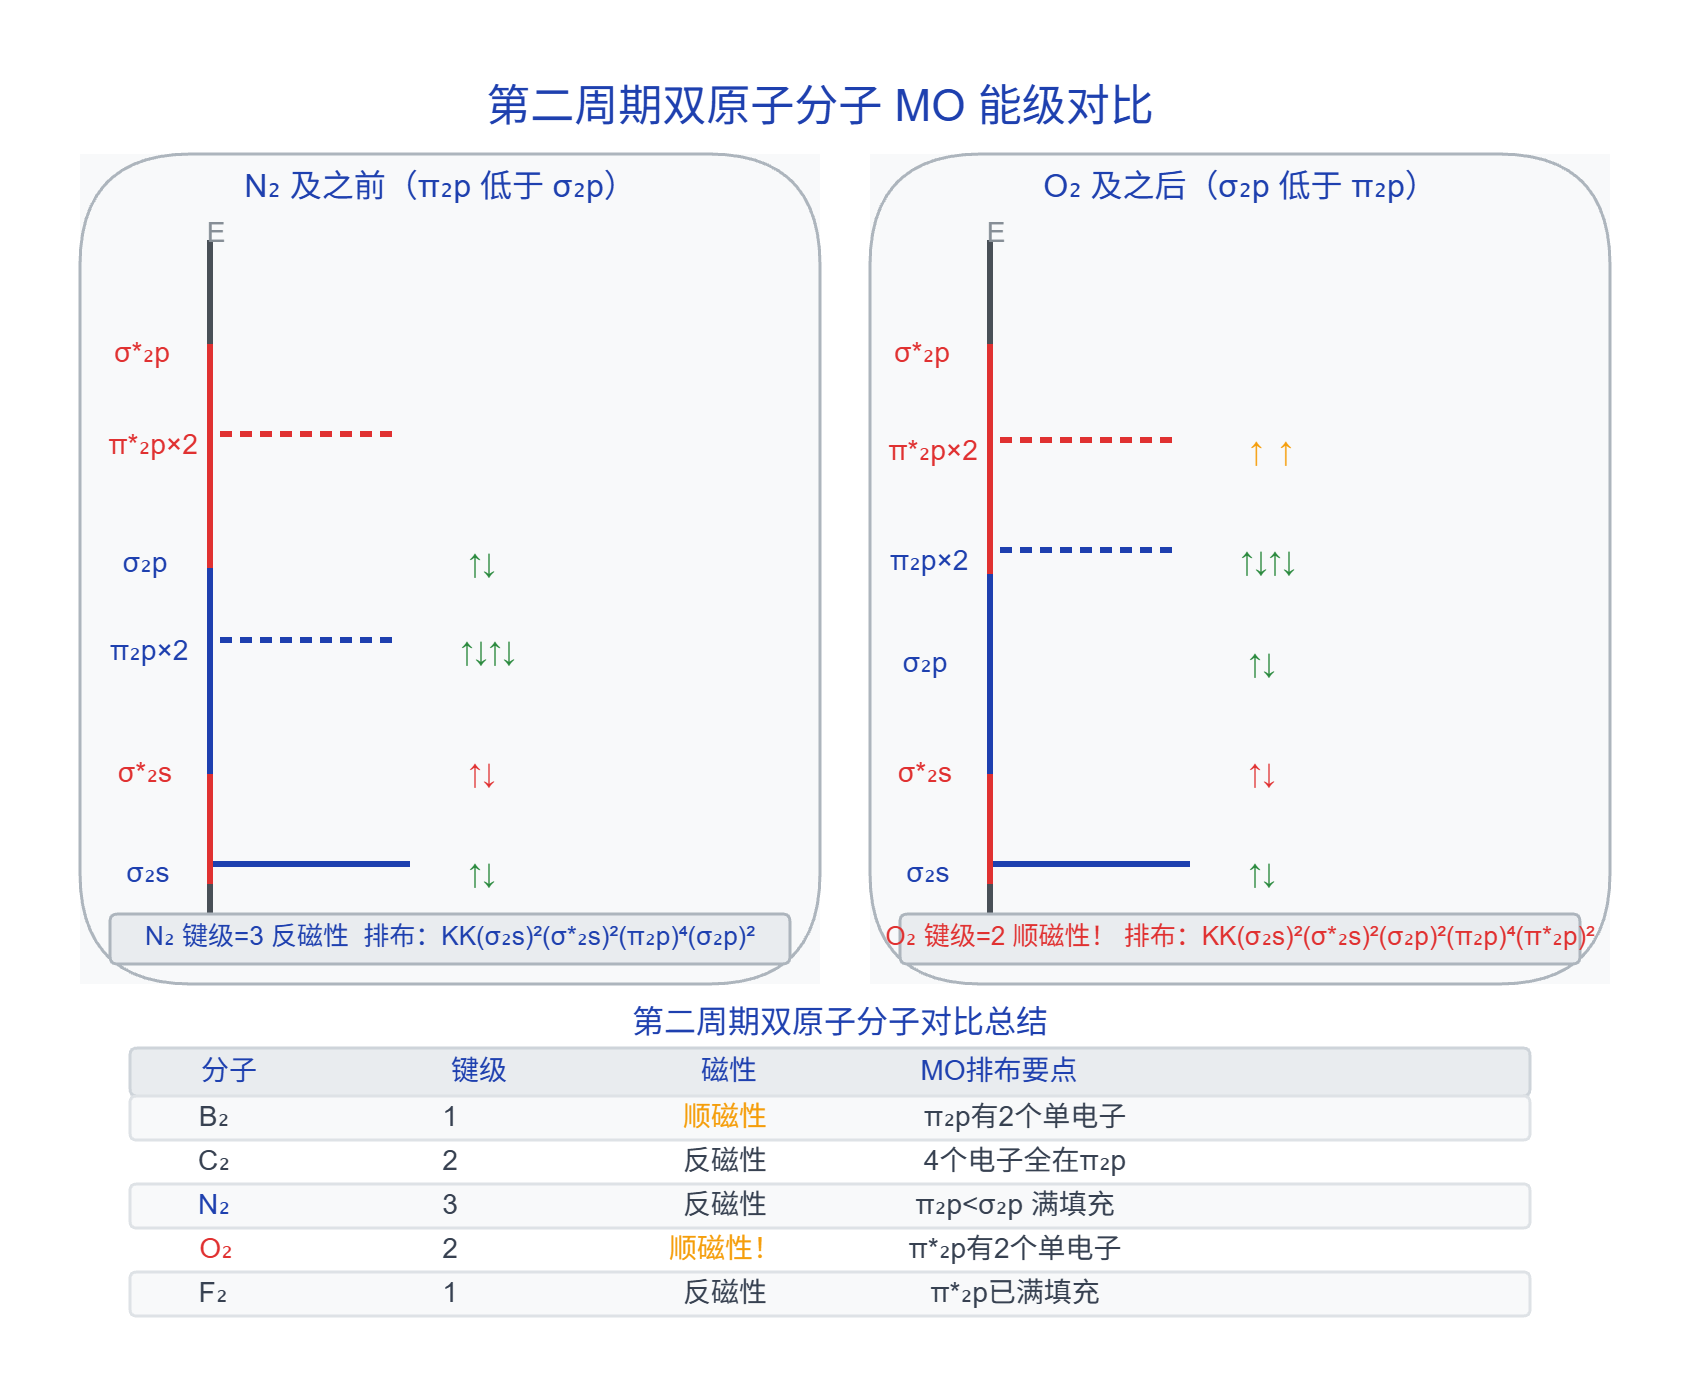
\includegraphics[width=0.45\textwidth,keepaspectratio]{media/h2-energy-curve.jpg}
\caption{H 分子的势能曲线—为什么存在最佳键长}
\end{figure}

\textbf{H\textsubscript{2} 势能曲线的三个关键区域}：
- \textbf{r 很大}(原子相距远)：相互作用弱，势能 \约等于 0
- \textbf{r = r\textsubscript{0}(平衡键长，0.74 Å)}：势能最低(-436 kJ/mol)，\textbf{这是最稳定的状态}
- \textbf{r \textless{} r\textsubscript{0}}(原子太近)：核间排斥急剧上升，势能飙升

\textbf{教学洞察}：``为什么原子不会无限靠近？''---这是质心教学逻辑中的\textbf{首个认知冲突}。答案是：电子云重叠降低了动能，但核间排斥在短距离急剧增大。两股力量平衡\箭存在最佳键长 r\textsubscript{0}。

\textbf{\西格马 键与 \派 键}：共价键按轨道重叠方式分为两类：

\begin{figure}[H]\centering
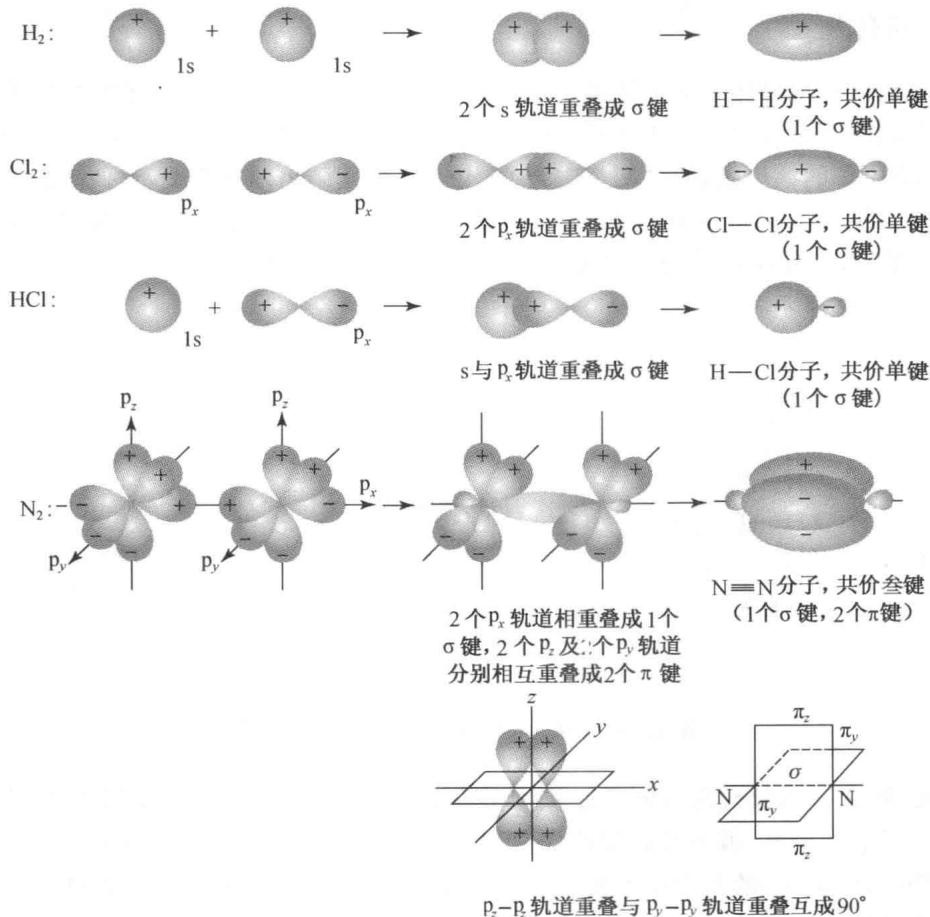
\includegraphics[width=0.45\textwidth,keepaspectratio]{media/sigma-pi-bond-formation.jpg}
\caption{键(头对头重叠)与 键(肩并肩重叠)的形成方式}
\end{figure}

{\def\LTcaptype{none} % do not increment counter
\begin{longtable}[]{@{}
  >{\raggedright\arraybackslash}p{(\linewidth - 8\tabcolsep) * \real{0.2000}}
  >{\raggedright\arraybackslash}p{(\linewidth - 8\tabcolsep) * \real{0.2000}}
  >{\raggedright\arraybackslash}p{(\linewidth - 8\tabcolsep) * \real{0.2000}}
  >{\raggedright\arraybackslash}p{(\linewidth - 8\tabcolsep) * \real{0.2000}}
  >{\raggedright\arraybackslash}p{(\linewidth - 8\tabcolsep) * \real{0.2000}}@{}}
\toprule\noalign{}
\begin{minipage}[b]{\linewidth}\raggedright
重叠方式
\end{minipage} & \begin{minipage}[b]{\linewidth}\raggedright
键型
\end{minipage} & \begin{minipage}[b]{\linewidth}\raggedright
电子云分布
\end{minipage} & \begin{minipage}[b]{\linewidth}\raggedright
特点
\end{minipage} & \begin{minipage}[b]{\linewidth}\raggedright
实例
\end{minipage} \\
\midrule\noalign{}
\endhead
\bottomrule\noalign{}
\endlastfoot
\textbf{头对头}(沿键轴方向) & \西格马 键 & 圆柱对称，沿键轴集中 & 键能大、可自由旋转 & H\textsubscript{2}、C-C 单键 \\
\textbf{肩并肩}(垂直于键轴) & \派 键 & 上下两片分布于键轴两侧 & 键能小、不可旋转 & C=C 中的第二个键 \\
\end{longtable}
}

\textbf{记忆口诀}：``\西格马 头碰头，\派 肩并肩。\西格马 可转，\派 不转。''

\textbf{共价键的两个关键特征}：
- \textbf{饱和性}：每个原子能形成的共价键数目有限(受可用轨道和电子数限制)。例如 H 最多 1 个键(只有 1s)，O 最多 2 个键(2 个未成对电子)。
- \textbf{方向性}：共价键在特定方向形成(轨道重叠有方向性)，这决定了分子的空间构型。

\subsubsection{1.5 配位键 --- 特殊的共价键}\label{ux914dux4f4dux952e-ux7279ux6b8aux7684ux5171ux4ef7ux952e}

配位键是共价键的一种特殊形式：\textbf{成键电子对由一方原子单独提供}，另一方提供空轨道。

\[
\text{A} : + \text{B} \longrightarrow \text{A} \rightarrow \text{B}
\]

其中 A 为电子对给体(donor)，B 为电子对受体(acceptor)。

\begin{figure}[H]\centering
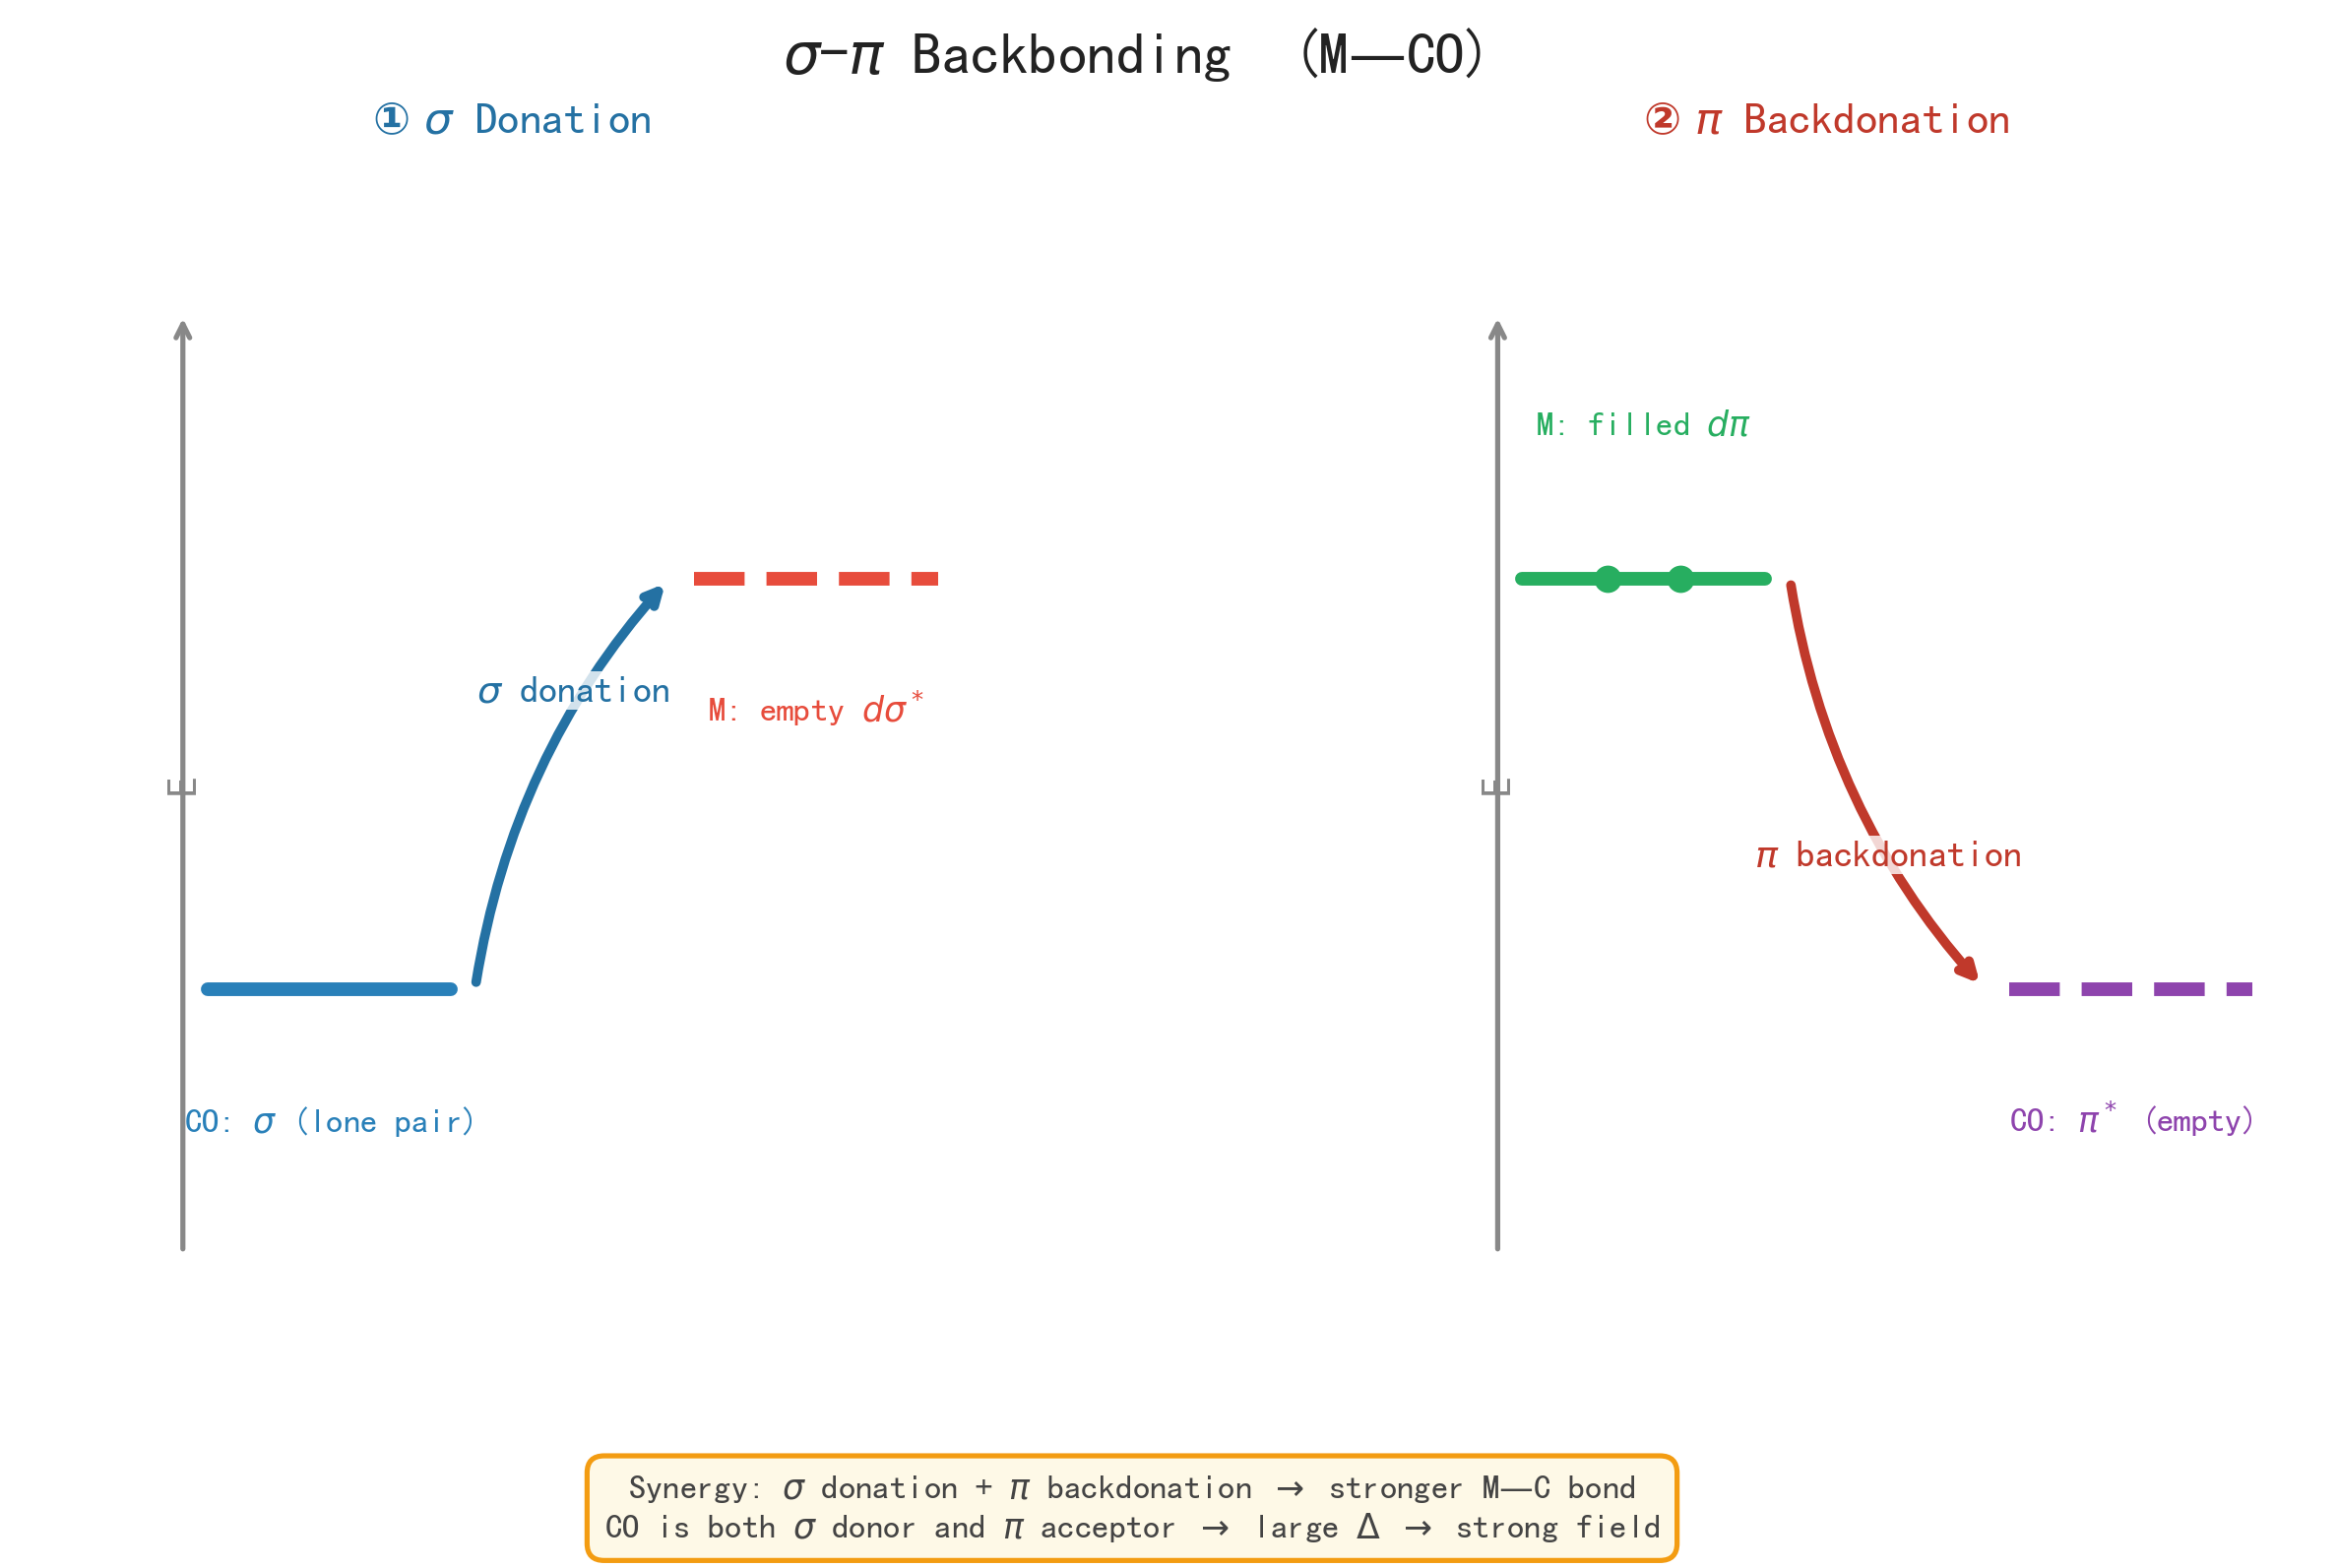
\includegraphics[width=0.45\textwidth,keepaspectratio]{media/sigma-pi-backbonding.png}
\caption{给予/-反馈协同机制}
\end{figure}

\textbf{\西格马-给予/\派-反馈协同}(在过渡金属配合物中尤为重要)：
- \textbf{\西格马-给予}：配体的孤对电子\箭金属的空 d 轨道(配体\箭金属)
- \textbf{\派-反馈}：金属的 d 电子\箭配体的 \派* 反键轨道(金属\箭配体)
- 两者协同增强配位键强度：\西格马 给予使金属电子密度增加\箭促进 \派 反馈\箭\派 反馈又促进 \西格马 给予

\textbf{应用}：CO 与过渡金属的配位就依赖 \西格马-给予/\派-反馈协同---这也是为什么 CO 是极强的场配体。

相关知识点：化学键

\begin{center}\rule{0.5\linewidth}{0.5pt}\end{center}

\subsection{二、Lewis 结构 --- 成键的语言}\label{ux4e8clewis-ux7ed3ux6784-ux6210ux952eux7684ux8bedux8a00}

\subsubsection{2.1 为什么从 Lewis 结构开始？}\label{ux4e3aux4ec0ux4e48ux4ece-lewis-ux7ed3ux6784ux5f00ux59cb}

化学的本质是\textbf{原子的重新组合}，而原子之间靠''键''连接。要理解分子为什么是某个形状、为什么有特定性质，第一步就是问：\textbf{原子之间有多少个键？电子在哪儿？}

Lewis 结构用最简单的语言---\textbf{共用电子对}---来回答这个问题。它不涉及复杂的量子力学，只需要数电子、画点线，就能告诉我们：
- 分子中有多少化学键(单键/双键/三键)
- 哪些原子有孤对电子(孤对电子影响形状！)
- 哪个共振结构贡献最大(形式电荷的妙用)

\textbf{核心假设}：原子通过共用电子对达到稀有气体电子构型(八隅体规则)。

\textbf{教学洞察}：Lewis 结构虽然是''最简单的''模型，但它是一切后续讨论的基础。VSEPR 需要它提供电子对数目，杂化轨道需要它判断 \西格马 键数，离域\派键需要它确定未参与杂化的 p 轨道和孤对电子数。\textbf{学好 Lewis 结构，整个分子结构章节就通了 50\%。}

{\def\LTcaptype{none} % do not increment counter
\begin{longtable}[]{@{}lll@{}}
\toprule\noalign{}
原子 & 目标构型 & 说明 \\
\midrule\noalign{}
\endhead
\bottomrule\noalign{}
\endlastfoot
H & 2e\textsuperscript{-}(He 型) & 唯一例外 \\
第二周期(C/N/O/F) & 8e\textsuperscript{-}(Ne 型) & 严格遵循八隅体 \\
第三周期及以后 & 可超过 8e\textsuperscript{-} & 利用 d 轨道扩展 \\
\end{longtable}
}

\subsubsection{2.2 Lewis 结构书写 --- 五步法}\label{lewis-ux7ed3ux6784ux4e66ux5199-ux4e94ux6b65ux6cd5}

\begin{Shaded}
\begin{Highlighting}[]
\NormalTok{Step 1: 算总价电子数 S}
\NormalTok{  S = 各原子价电子数之和 ± 离子电荷}
\NormalTok{  口诀：S = N (总价电子) {-} A (骨架单键用去)}

\NormalTok{Step 2: 确定骨架}
\NormalTok{  电负性小的原子居中，H 和卤素永远在端基}

\NormalTok{Step 3: 单键连接骨架，用去 2e⁻/键}
\NormalTok{  剩余电子优先满足端基原子的八隅体}

\NormalTok{Step 4: 若中心原子未满足八隅体，将端基孤对电子改为多重键}

\NormalTok{Step 5: 算形式电荷，选最优结构}
\end{Highlighting}
\end{Shaded}

\textbf{例}：NO\textsubscript{3}\textsuperscript{-} 的 Lewis 结构
- S = N(5) + O(6×3) + 1(负电荷) = 24 个价电子
- 骨架：N 居中，3 个 O 在端基
- 3 个 N-O 单键用去 6e\textsuperscript{-}，剩余 18e\textsuperscript{-} \箭 3 个 O 各分 6e\textsuperscript{-}(3 对孤对)
- N 只有 6e\textsuperscript{-} \箭 将一个 O 的 1 对孤对改为双键 \箭 N 达到 8e\textsuperscript{-}

\textbf{练习：Lewis 五步法补全表}

{\def\LTcaptype{none} % do not increment counter
\begin{longtable}[]{@{}
  >{\centering\arraybackslash}p{(\linewidth - 8\tabcolsep) * \real{0.2083}}
  >{\centering\arraybackslash}p{(\linewidth - 8\tabcolsep) * \real{0.2083}}
  >{\raggedright\arraybackslash}p{(\linewidth - 8\tabcolsep) * \real{0.1667}}
  >{\centering\arraybackslash}p{(\linewidth - 8\tabcolsep) * \real{0.2083}}
  >{\centering\arraybackslash}p{(\linewidth - 8\tabcolsep) * \real{0.2083}}@{}}
\toprule\noalign{}
\begin{minipage}[b]{\linewidth}\centering
分子/离子
\end{minipage} & \begin{minipage}[b]{\linewidth}\centering
总价电子数 S
\end{minipage} & \begin{minipage}[b]{\linewidth}\raggedright
骨架
\end{minipage} & \begin{minipage}[b]{\linewidth}\centering
中心是否满足八隅体？
\end{minipage} & \begin{minipage}[b]{\linewidth}\centering
是否有孤对？
\end{minipage} \\
\midrule\noalign{}
\endhead
\bottomrule\noalign{}
\endlastfoot
CO\textsubscript{2} & 16 & O-C-O & {[}完成{]} & 每个 O 有 2 对孤对 \\
SO\textsubscript{2} & \_\_\_\_ & \_\_\_\_ & \_\_\_\_ & \_\_\_\_ \\
ClO\textsubscript{4}\textsuperscript{-} & \_\_\_\_ & \_\_\_\_ & \_\_\_\_ & \_\_\_\_ \\
BrF\textsubscript{3} & \_\_\_\_ & \_\_\_\_ & \_\_\_\_ & \_\_\_\_ \\
\end{longtable}
}

答案见 §十二''课堂练习参考答案''。

\subsubsection{2.2b 键数公式 --- 画 Lewis 结构前的''秒算''工具}\label{b-ux952eux6570ux516cux5f0f-ux753b-lewis-ux7ed3ux6784ux524dux7684ux79d2ux7b97ux5de5ux5177}

竞赛中遇到陌生分子，第一步不是凭感觉画，而是 \textbf{``先算键数，再画骨架''}。

\[
n_{\text{键}} = \frac{1}{2}\left(\sum n_{\text{希望得到的电子数}} - \sum n_{\text{价电子数}}\right)
\]

\textbf{逻辑}：每个原子希望达到稀有气体构型需要多少电子，减去实际有多少价电子，差额就是要通过成键补足的电子数，除以 2 = 键数。

\begin{itemize}
\tightlist
\item
  H 希望 2 电子，其他主族原子希望 8 电子
\item
  含配位键时：受体''多得 2 个电子''，给体不变
\item
  \textbf{例}：N\textsubscript{8} 链状分子 \箭 \(8 \times (8-5) / 2 = 12\) 根键，秒算
\end{itemize}

\textbf{课堂提示}：``先算键数，再画骨架''，避免''画了又改''的反复。

\begin{center}\rule{0.5\linewidth}{0.5pt}\end{center}

\subsubsection{2.3 形式电荷(Formal Charge)}\label{ux5f62ux5f0fux7535ux8377formal-charge}

\[
\text{FC} = \text{价电子数} - \text{孤对电子数} - \frac{1}{2} \times \text{成键电子数}
\]

\textbf{三规则口诀版}(快速校验)：

{\def\LTcaptype{none} % do not increment counter
\begin{longtable}[]{@{}
  >{\raggedright\arraybackslash}p{(\linewidth - 4\tabcolsep) * \real{0.3333}}
  >{\raggedright\arraybackslash}p{(\linewidth - 4\tabcolsep) * \real{0.3333}}
  >{\raggedright\arraybackslash}p{(\linewidth - 4\tabcolsep) * \real{0.3333}}@{}}
\toprule\noalign{}
\begin{minipage}[b]{\linewidth}\raggedright
规则
\end{minipage} & \begin{minipage}[b]{\linewidth}\raggedright
口诀
\end{minipage} & \begin{minipage}[b]{\linewidth}\raggedright
说明
\end{minipage} \\
\midrule\noalign{}
\endhead
\bottomrule\noalign{}
\endlastfoot
\textbf{规则 1} & 成键数 = 族数 \箭 FC = 0 & 特征键数 = 族数(如 N 族数 5，特征键数 3) \\
\textbf{规则 2} & 多一根键 \箭 FC +1 & 自己的电子被迫分给别人了 \\
\textbf{规则 3} & 少一根键 \箭 FC −1 & 从别人那里多得了电子 \\
\textbf{校验} & 所有 FC 之和 = 物种净电荷 & 画完必查，避免漏算 \\
\end{longtable}
}

\textbf{记忆口诀}：``成键数=族数\箭FC=0；多一根键\箭FC+1；少一根键\箭FC−1；和等于净电荷。''

\textbf{最优结构选择原则}(按优先级)：
1. 形式电荷绝对值之和最小
2. 负电荷在电负性大的原子上
3. 避免同号电荷在相邻原子上

\textbf{教学洞察}：中文化学命名中的''形式电荷''常译作''形式电荷''，但这个''形式''二字正是最大的误导源---学生最容易犯的错误就是认为形式电荷就是该原子的实际电荷。\textbf{FC = -1 不意味着该原子带 1 个负电荷，它只是一个人为分配的''表观电荷''，用来在不同共振结构之间做比较的。} CO 分子中 C 的形式电荷为 -1、O 为 +1，但实验测得 CO 的偶极矩方向为 C\textsuperscript{-}\箭O\textsuperscript{+} 吗？非也---实际 CO 的偶极矩极小且方向是 C\textsuperscript{+}\箭O\textsuperscript{-}。这就证明形式电荷 \不等于 实际电荷。

\textbf{易错提醒}：形式电荷计算中，\textbf{孤对电子数和成键电子数要分清楚}。初学者常见错误是：将双键的 4 个电子全部计入''成键电子''，但公式中的''成键电子数''指的是与该原子直接相连的共价键中的总电子数---双键算 4 个。公式为 \(\text{FC} = \text{价电子数} - \text{孤对电子数} - \frac{1}{2} \times \text{成键电子数}\)。

\subsubsection{2.4 共振结构}\label{ux5171ux632fux7ed3ux6784}

当单个 Lewis 结构无法准确描述电子分布时，需要多个 Lewis 结构共同描述---\textbf{共振杂化体}。

\textbf{书写要点}：
- 各共振式中原子位置固定(不是同分异构体)
- 各共振式中孤对电子数相等
- 形式电荷为 0 的结构最稳定

\textbf{五条稳定性判据}(按重要度排序，逐条筛选)：

{\def\LTcaptype{none} % do not increment counter
\begin{longtable}[]{@{}cll@{}}
\toprule\noalign{}
优先级 & 判据 & 说明 \\
\midrule\noalign{}
\endhead
\bottomrule\noalign{}
\endlastfoot
1 & \textbf{满足八隅体} & 最重要，不满足直接排除 \\
2 & \textbf{FC 绝对值 \小于等于 1} & FC = ±2 的结构通常不稳定 \\
3 & \textbf{电负性匹配} & 电负性高的原子不承受正 FC \\
4 & \textbf{键数尽可能多} & 键能高 = 更稳定 \\
5 & \textbf{正负 FC 相邻} & 静电吸引贡献额外稳定化 \\
\end{longtable}
}

\textbf{课堂速查}：按 1\箭5 逐条筛，第一条不满足直接排除，不必全看完再回头。

\textbf{例}：SCN\textsuperscript{-} 的共振结构

{\def\LTcaptype{none} % do not increment counter
\begin{longtable}[]{@{}
  >{\raggedright\arraybackslash}p{(\linewidth - 6\tabcolsep) * \real{0.2353}}
  >{\raggedright\arraybackslash}p{(\linewidth - 6\tabcolsep) * \real{0.2353}}
  >{\centering\arraybackslash}p{(\linewidth - 6\tabcolsep) * \real{0.2941}}
  >{\raggedright\arraybackslash}p{(\linewidth - 6\tabcolsep) * \real{0.2353}}@{}}
\toprule\noalign{}
\begin{minipage}[b]{\linewidth}\raggedright
结构
\end{minipage} & \begin{minipage}[b]{\linewidth}\raggedright
形式电荷
\end{minipage} & \begin{minipage}[b]{\linewidth}\centering
是否满足八隅体
\end{minipage} & \begin{minipage}[b]{\linewidth}\raggedright
优劣
\end{minipage} \\
\midrule\noalign{}
\endhead
\bottomrule\noalign{}
\endlastfoot
{[}S---C≡N{]}\textsuperscript{-} & S(−1), C(0), N(0) & 是 & 负电荷在 S 上(电负性较小) \\
{[}S=C=N{]}\textsuperscript{-} & S(0), C(0), N(−1) & 是 & \textbf{最优}---负电荷在电负性更大的 N 上 \\
{[}S≡C---N{]}\textsuperscript{2-} & S(0), C(−1), N(−1) & 是 & FC 绝对值超出±1，不稳定 \\
\end{longtable}
}

\textbf{例}：NO\textsubscript{3}\textsuperscript{-} 的三个等价共振结构：

实际 N-O 键长均等(介于单键和双键之间)，说明电子离域到整个 NO\textsubscript{3}\textsuperscript{-} 离子中。

\subsubsection{2.5 Lewis 结构式的局限性}\label{lewis-ux7ed3ux6784ux5f0fux7684ux5c40ux9650ux6027}

Lewis 结构式是理解分子结构的基础工具，但它不能解释以下现象---这些需要后续的价键理论和分子轨道理论来补充：

{\def\LTcaptype{none} % do not increment counter
\begin{longtable}[]{@{}
  >{\raggedright\arraybackslash}p{(\linewidth - 6\tabcolsep) * \real{0.2353}}
  >{\raggedright\arraybackslash}p{(\linewidth - 6\tabcolsep) * \real{0.2353}}
  >{\raggedright\arraybackslash}p{(\linewidth - 6\tabcolsep) * \real{0.2353}}
  >{\centering\arraybackslash}p{(\linewidth - 6\tabcolsep) * \real{0.2941}}@{}}
\toprule\noalign{}
\begin{minipage}[b]{\linewidth}\raggedright
局限
\end{minipage} & \begin{minipage}[b]{\linewidth}\raggedright
说明
\end{minipage} & \begin{minipage}[b]{\linewidth}\raggedright
实例
\end{minipage} & \begin{minipage}[b]{\linewidth}\centering
补充理论
\end{minipage} \\
\midrule\noalign{}
\endhead
\bottomrule\noalign{}
\endlastfoot
共价键的本质 & 为什么共用电子对能使原子结合？ & H\textsubscript{2} 的共价键 & 价键理论(轨道重叠) \\
O\textsubscript{2} 的顺磁性 & Lewis 式所有电子配对\箭应为反磁性 & O\textsubscript{2} 有 2 个未成对电子 & 分子轨道理论 \\
键长平均化 & 共振解释后需理解''共振杂化体'' & 苯的 6 个 C-C 键等长(139pm) & 共振论/分子轨道 \\
超价化合物 & 第三周期起 d 轨道可参与成键 & PCl\textsubscript{5}(10e), SF\textsubscript{6}(12e) & 杂化轨道理论 \\
缺电子分子 & 中心原子不满八隅体 & BF\textsubscript{3}(6e), BeCl\textsubscript{2}(4e) & 价键理论(三中心键) \\
\end{longtable}
}

\textbf{历史地位}：Lewis 八隅体规则(1916 年)能解释大量主族元素化合物的成键，至今仍是分子结构分析的第一入门工具。但它只是''近似''而不是''真理''---后续各讲将逐一克服它的局限。

\begin{center}\rule{0.5\linewidth}{0.5pt}\end{center}

\subsection{三、VSEPR 理论 --- 猜形状}\label{ux4e09vsepr-ux7406ux8bba-ux731cux5f62ux72b6}

为什么 Lewis 结构还不够？因为知道电子怎么连只是第一步---我们还需要知道分子在\textbf{三维空间里长什么样}。NH\textsubscript{3} 是平面三角形还是三角锥形？这决定了它有没有极性(NH\textsubscript{3} 是极性分子，BF\textsubscript{3} 是非极性)。

VSEPR 理论的价值就在于此：\textbf{从 Lewis 结构中的电子对数目，推断分子的三维形状。} 它不考虑复杂的量子力学，只用''电子对互相排斥''这一条直觉，就能准确预测绝大多数分子的构型---包括很多''反直觉''的情况(比如 XeF\textsubscript{2} 明明是三个原子却是直线形)。

\textbf{关键定位}：VSEPR 是''描述性''理论---它告诉我们\textbf{是什么形状}，但不告诉我们\textbf{为什么是这个形状}。后面的杂化轨道理论才回答''为什么''。

\subsubsection{3.1 核心思想}\label{ux6838ux5fc3ux601dux60f3}

\textbf{价层电子对互斥理论}：价层电子对(成键电子对 + 孤对电子)互相排斥，趋向于尽可能远离。

\subsubsection{3.2 AXₙEₘ 模型}\label{axux2099eux2098-ux6a21ux578b}

\begin{itemize}
\tightlist
\item
  A = 中心原子
\item
  X = 配位原子(成键电子对)
\item
  E = 孤对电子
\item
  n + m = 价层电子对总数
\end{itemize}

{\def\LTcaptype{none} % do not increment counter
\begin{longtable}[]{@{}clllcl@{}}
\toprule\noalign{}
总电子对数 & 理想排布 & 分子类型 & 实际构型 & 键角 & 实例 \\
\midrule\noalign{}
\endhead
\bottomrule\noalign{}
\endlastfoot
2 & 直线形 & AX\textsubscript{2} & 直线形 & 180° & BeCl\textsubscript{2}、CO\textsubscript{2} \\
3 & 平面三角形 & AX\textsubscript{3} & 平面三角形 & 120° & BF\textsubscript{3}、NO\textsubscript{3}\textsuperscript{-} \\
& & AX\textsubscript{2}E & V 形 & \textless120° & SO\textsubscript{2}、O\textsubscript{3} \\
4 & 四面体 & AX\textsubscript{4} & 四面体 & 109.5° & CH\textsubscript{4}、NH\textsubscript{4}\textsuperscript{+} \\
& & AX\textsubscript{3}E & 三角锥形 & \textless109.5° & NH\textsubscript{3}(107°) \\
& & AX\textsubscript{2}E\textsubscript{2} & V 形 & \textless109.5° & H\textsubscript{2}O(104.5°) \\
5 & 三角双锥 & AX\textsubscript{5} & 三角双锥 & 90°/120° & PCl\textsubscript{5} \\
& & AX\textsubscript{4}E & 跷跷板形 & --- & SF\textsubscript{4} \\
& & AX\textsubscript{3}E\textsubscript{2} & T 形 & --- & ClF\textsubscript{3} \\
& & AX\textsubscript{2}E\textsubscript{3} & 直线形 & --- & XeF\textsubscript{2} \\
6 & 八面体 & AX\textsubscript{6} & 八面体 & 90° & SF\textsubscript{6} \\
& & AX\textsubscript{5}E & 四方锥形 & --- & BrF\textsubscript{5} \\
& & AX\textsubscript{4}E\textsubscript{2} & 平面正方形 & --- & XeF\textsubscript{4} \\
\end{longtable}
}

\begin{figure}[H]\centering
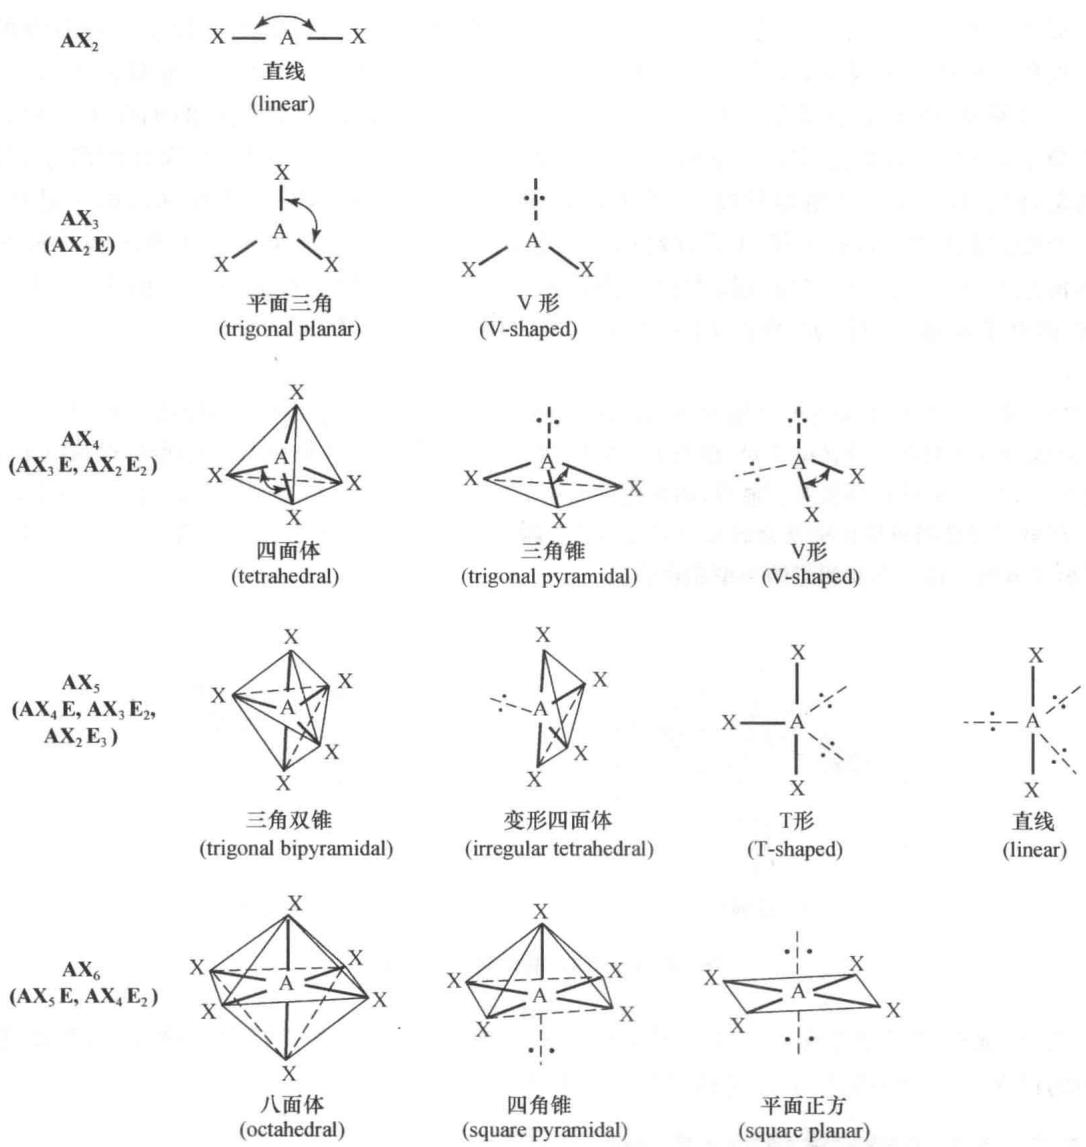
\includegraphics[width=0.45\textwidth,keepaspectratio]{media/12-21-vsepr-ax5-ax6-molecular-geometries.jpg}
\caption{VSEPR 常见构型汇总(AX-AX)}
\end{figure}

\textbf{练习：VSEPR 模型补全表}

{\def\LTcaptype{none} % do not increment counter
\begin{longtable}[]{@{}
  >{\centering\arraybackslash}p{(\linewidth - 12\tabcolsep) * \real{0.1515}}
  >{\centering\arraybackslash}p{(\linewidth - 12\tabcolsep) * \real{0.1515}}
  >{\centering\arraybackslash}p{(\linewidth - 12\tabcolsep) * \real{0.1515}}
  >{\centering\arraybackslash}p{(\linewidth - 12\tabcolsep) * \real{0.1515}}
  >{\centering\arraybackslash}p{(\linewidth - 12\tabcolsep) * \real{0.1515}}
  >{\raggedright\arraybackslash}p{(\linewidth - 12\tabcolsep) * \real{0.1212}}
  >{\raggedright\arraybackslash}p{(\linewidth - 12\tabcolsep) * \real{0.1212}}@{}}
\toprule\noalign{}
\begin{minipage}[b]{\linewidth}\centering
分子
\end{minipage} & \begin{minipage}[b]{\linewidth}\centering
总电子对数
\end{minipage} & \begin{minipage}[b]{\linewidth}\centering
成键数 n
\end{minipage} & \begin{minipage}[b]{\linewidth}\centering
孤对数 m
\end{minipage} & \begin{minipage}[b]{\linewidth}\centering
AXₙEₘ
\end{minipage} & \begin{minipage}[b]{\linewidth}\raggedright
理想排布
\end{minipage} & \begin{minipage}[b]{\linewidth}\raggedright
实际构型
\end{minipage} \\
\midrule\noalign{}
\endhead
\bottomrule\noalign{}
\endlastfoot
SF\textsubscript{4} & 5 & 4 & 1 & AX\textsubscript{4}E & 三角双锥 & 跷跷板形 \\
ClF\textsubscript{3} & \_\_\_\_ & \_\_\_\_ & \_\_\_\_ & \_\_\_\_ & \_\_\_\_ & \_\_\_\_ \\
XeF\textsubscript{2} & \_\_\_\_ & \_\_\_\_ & \_\_\_\_ & \_\_\_\_ & \_\_\_\_ & \_\_\_\_ \\
IF\textsubscript{4}\textsuperscript{-} & \_\_\_\_ & \_\_\_\_ & \_\_\_\_ & \_\_\_\_ & \_\_\_\_ & \_\_\_\_ \\
\end{longtable}
}

提示：先算中心原子的价层电子总数(考虑配体贡献和离子电荷)，÷2 得电子对数，再减去成键数得孤对数。

\subsubsection{3.3 关键规则}\label{ux5173ux952eux89c4ux5219}

\textbf{孤对电子的位置选择}：
- 在三角双锥体系(5 对电子)中，孤对电子\textbf{优先占据赤道向位置}(夹角 120°，空间更大)，而非轴向位置(夹角 90°，排斥更强)。
- 记忆口诀：\textbf{``孤对先占赤道位，90° 最少为赢''}
- 类比：\textbf{``大胖子(孤对电子)坐赤道位，旁边只要忍受 2 个 90° 的人；坐轴向位要忍 3 个。''}

\textbf{教学洞察}：孤对电子的位置选择是最容易被忽视的高频考点。SF\textsubscript{4}(AX\textsubscript{4}E，跷跷板形)中孤对放赤道位、ClF\textsubscript{3}(AX\textsubscript{3}E\textsubscript{2}，T 形)中两对孤对都放赤道位---记忆核心不是背形状，而是理解''最小化 90° 排斥''原则。对于 5 对电子的三角双锥体系，\textbf{孤对优先占赤道 \箭 赤道位留给孤对 \箭 轴向位留给配体}。

\textbf{排斥力大小顺序}：
\[
\text{孤对–孤对} > \text{孤对–成键} > \text{成键–成键}
\]

\textbf{易错提醒}：NH\textsubscript{3} 的键角为什么是 107° 而非 109.5°？因为 1 对孤对的排斥 \textgreater{} 1 个成键对的排斥 \箭 孤对压缩 H-N-H 键角。H\textsubscript{2}O 更狠---2 对孤对！压缩到 104.5°。\textbf{每多 1 对孤对，键角被压缩约 2°--2.5°}(粗略估算，但有用)。

\textbf{多重键的处理}：多重键视为 \textbf{1 个电子对区域}。例如 CO\textsubscript{2} 中 C 与 O 各形成一个双键，共 2 个电子对区域 \箭 直线形。

\textbf{常见误解}：双键有 4 个电子，三键有 6 个电子---为什么在 VSEPR 中都只算 1 个区域？因为这些电子都在\textbf{同一方向}(都在键轴上或都在垂直于键轴的方向上)，它们的排斥效应等价于 1 组电子对。记忆：\textbf{``多重键的电子对都在同一方向怼你，算 1 组就够了。''}

相关知识点：VSEPR理论

\subsubsection{3.4 分子极性判断 --- 三步法}\label{ux5206ux5b50ux6781ux6027ux5224ux65ad-ux4e09ux6b65ux6cd5}

VSEPR 预测了分子形状，结合键的极性就能判断分子极性。

\textbf{三步判断法}：
1. \textbf{看键}：是否有极性键(Δχ \textgreater{} 0)？\箭 无则非极性分子
2. \textbf{看形}：分子构型是否对称？\箭 对称则键矩抵消
3. \textbf{看矢量和}：所有键偶极矩的矢量和是否为零？\箭 零则非极性

\textbf{核心原则}：极性键是极性分子的必要条件，但不是充分条件。

\textbf{经典判断表}：

{\def\LTcaptype{none} % do not increment counter
\begin{longtable}[]{@{}lclcc@{}}
\toprule\noalign{}
分子 & 键的极性 & 构型 & 对称性 & 分子极性 \\
\midrule\noalign{}
\endhead
\bottomrule\noalign{}
\endlastfoot
CO\textsubscript{2} & C=O 极性键 & 直线形 AX\textsubscript{2} & 对称 & \textbf{非极性} \\
SO\textsubscript{2} & S=O 极性键 & V 形 AX\textsubscript{2}E & 不对称 & \textbf{极性} \\
BF\textsubscript{3} & B-F 极性键 & 平面三角形 AX\textsubscript{3} & 对称 & \textbf{非极性} \\
NH\textsubscript{3} & N-H 极性键 & 三角锥 AX\textsubscript{3}E & 不对称 & \textbf{极性} \\
CH\textsubscript{4} & C-H 弱极性键 & 正四面体 AX\textsubscript{4} & 对称 & \textbf{非极性} \\
CH\textsubscript{3}Cl & C-Cl 极性键 & 四面体(不对称取代) & 不对称 & \textbf{极性} \\
\end{longtable}
}

\textbf{高频考点}：CO\textsubscript{2}(非极性) vs SO\textsubscript{2}(极性)---只因孤电子对破坏了线性对称性。孤对电子本身不形成键，但\textbf{改变空间构型}，从而改变键偶极矩能否抵消。

\begin{center}\rule{0.5\linewidth}{0.5pt}\end{center}

\subsection{四、杂化轨道理论 --- 解释为什么}\label{ux56dbux6742ux5316ux8f68ux9053ux7406ux8bba-ux89e3ux91caux4e3aux4ec0ux4e48}

VSEPR 告诉我们分子''长什么样''，但没告诉我们\textbf{为什么}。为什么 CH\textsubscript{4} 是正四面体而不是平面正方形？为什么 H\textsubscript{2}O 的键角不是 90°(如果只用纯 p 轨道成键)而是 104.5°？

答案是：\textbf{电子轨道的''混合''}---杂化。

\textbf{关键定位}：VSEPR 是''描述性''理论(告诉我们是什么形状)，杂化轨道理论是''解释性''理论(告诉我们为什么是那个形状)。两者互相配合：先 VSEPR 预测形状，再杂化解释形状。\textbf{千万不要反过来}---不要从杂化类型推构型，而要从构型反推杂化类型。

\textbf{核心思想}：中心原子的能量相近的原子轨道(ns + np + nd)在成键过程中\textbf{线性组合}成数量相等、能量相同的\textbf{杂化轨道}，用于与配位原子成键。

\textbf{教学洞察}：学生最容易犯的概念性错误是把杂化当作原子的''固有属性''---他们问''CH\textsubscript{4} 中的 C 是什么杂化？``仿佛 C 原子天生就是 sp\textsuperscript{3} 杂化。\textbf{但杂化发生在成键过程中，不是原子固有的。} 孤立 C 原子的基态是 2s\textsuperscript{2}2p\textsuperscript{2}，只有在形成 4 个 C-H 键时，1 个 2s 电子被激发到 2p 空轨道，然后 1 个 2s + 3 个 2p 轨道杂化成 4 个 sp\textsuperscript{3} 杂化轨道---这是成键的''后果''，不是''前提''。
类比：\textbf{``混色---红色(s 轨道)+ 蓝色(p 轨道)\箭 紫色(sp 杂化轨道)。紫色既不是红也不是蓝，但包含了红和蓝的成分。而混合只是在你需要画画(成键)的时候才发生，不是颜料本身一直是混合的。''}

\subsubsection{4.1 杂化类型与几何构型}\label{ux6742ux5316ux7c7bux578bux4e0eux51e0ux4f55ux6784ux578b}

{\def\LTcaptype{none} % do not increment counter
\begin{longtable}[]{@{}clclcl@{}}
\toprule\noalign{}
杂化类型 & 参与轨道 & 杂化轨道数 & 空间构型 & 键角 & 实例 \\
\midrule\noalign{}
\endhead
\bottomrule\noalign{}
\endlastfoot
sp & s + p & 2 & 直线形 & 180° & BeCl\textsubscript{2}、CO\textsubscript{2} \\
sp\textsuperscript{2} & s + p + p & 3 & 平面三角形 & 120° & BF\textsubscript{3}、NO\textsubscript{3}\textsuperscript{-}、石墨 \\
sp\textsuperscript{3} & s + p + p + p & 4 & 四面体 & 109.5° & CH\textsubscript{4}、NH\textsubscript{3}、H\textsubscript{2}O \\
sp\textsuperscript{3}d & s + p + p + p + d & 5 & 三角双锥 & 90°/120° & PCl\textsubscript{5} \\
sp\textsuperscript{3}d\textsuperscript{2} & s + p + p + p + d + d & 6 & 八面体 & 90° & SF\textsubscript{6} \\
\end{longtable}
}

\begin{figure}[H]\centering
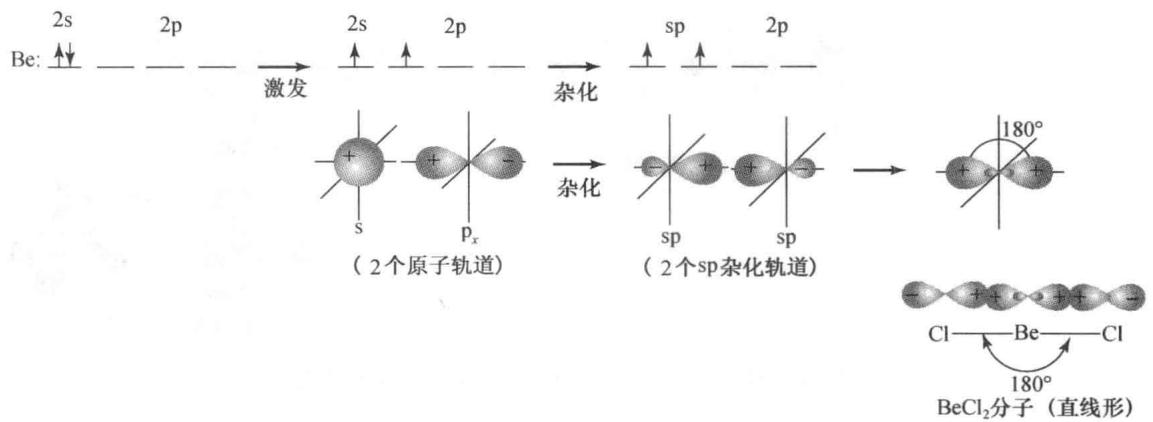
\includegraphics[width=0.3\textwidth,keepaspectratio]{media/12-7c-hybrid-orbital-formation-ch4-sp3.jpg}
\hspace{0.02\textwidth}
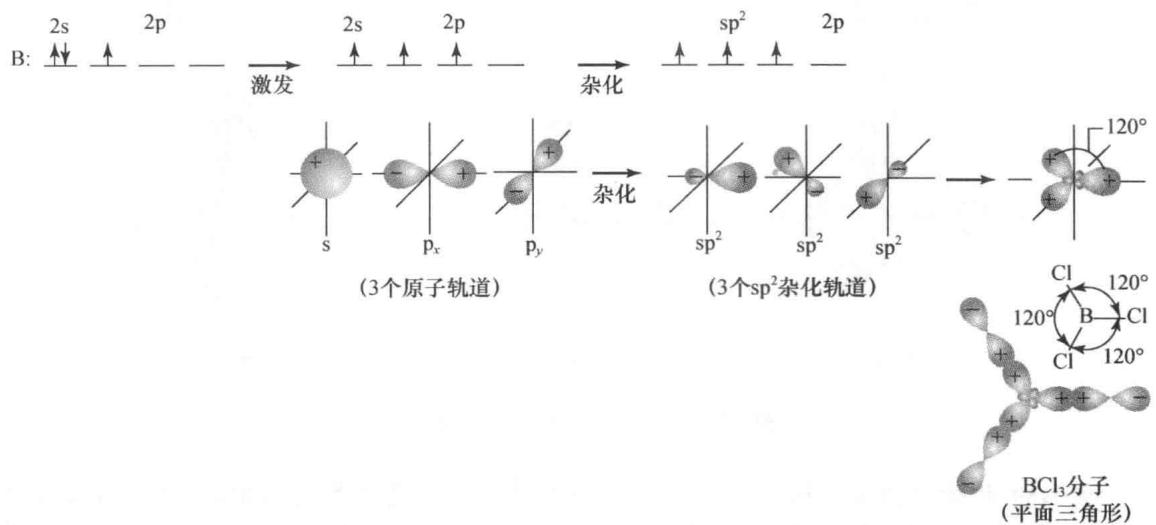
\includegraphics[width=0.3\textwidth,keepaspectratio]{media/12-7a-hybrid-orbital-formation-sp-sp2-sp3.jpg}
\hspace{0.02\textwidth}
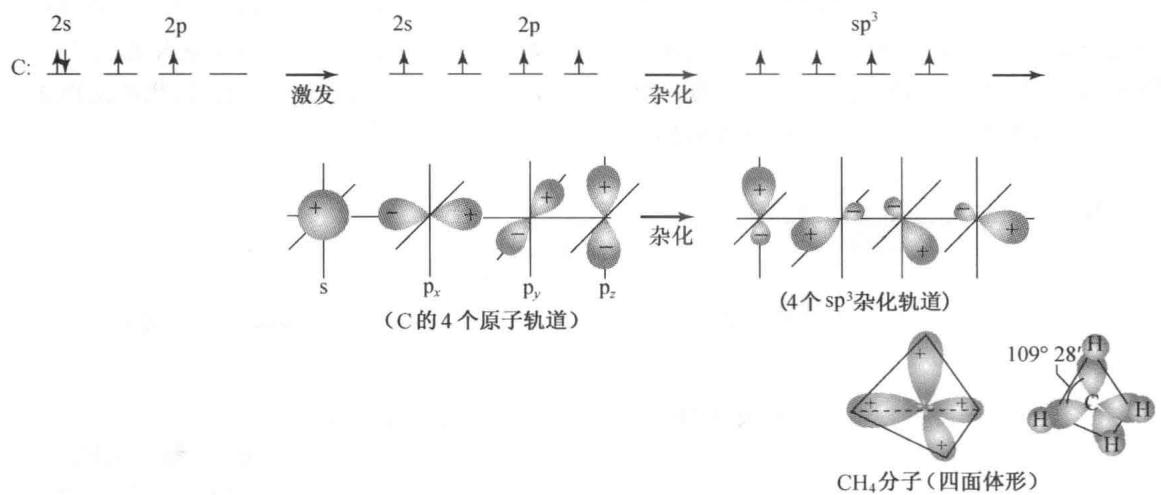
\includegraphics[width=0.3\textwidth,keepaspectratio]{media/12-7b-hybrid-orbital-formation-bcl3-sp2.jpg}
\caption{sp、sp、sp 杂化示意}
\end{figure}

\begin{figure}[H]\centering
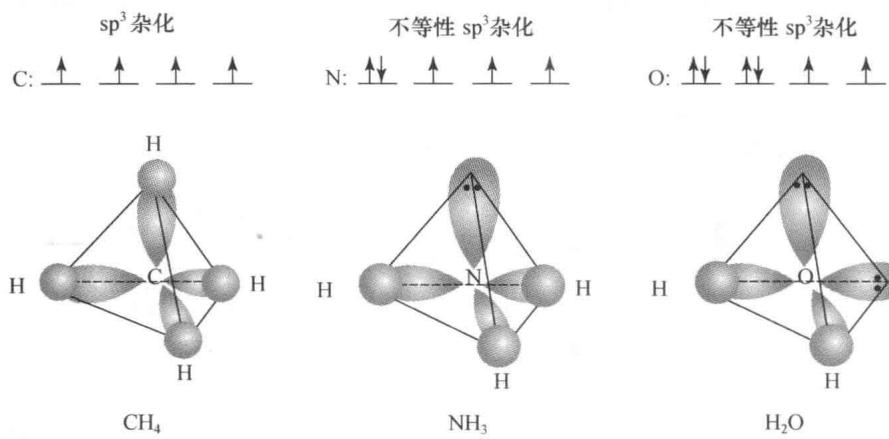
\includegraphics[width=0.45\textwidth,keepaspectratio]{media/12-8-ch4-nh3-h2o-bond-angle-comparison-sp3.jpg}
\caption{CH、NH、HO 的键角差异与孤对压缩}
\end{figure}

\subsubsection{4.2 等性杂化 vs 不等性杂化}\label{ux7b49ux6027ux6742ux5316-vs-ux4e0dux7b49ux6027ux6742ux5316}

{\def\LTcaptype{none} % do not increment counter
\begin{longtable}[]{@{}
  >{\raggedright\arraybackslash}p{(\linewidth - 8\tabcolsep) * \real{0.1905}}
  >{\raggedright\arraybackslash}p{(\linewidth - 8\tabcolsep) * \real{0.1905}}
  >{\raggedright\arraybackslash}p{(\linewidth - 8\tabcolsep) * \real{0.1905}}
  >{\centering\arraybackslash}p{(\linewidth - 8\tabcolsep) * \real{0.2381}}
  >{\raggedright\arraybackslash}p{(\linewidth - 8\tabcolsep) * \real{0.1905}}@{}}
\toprule\noalign{}
\begin{minipage}[b]{\linewidth}\raggedright
类型
\end{minipage} & \begin{minipage}[b]{\linewidth}\raggedright
特征
\end{minipage} & \begin{minipage}[b]{\linewidth}\raggedright
s/p 成分分布
\end{minipage} & \begin{minipage}[b]{\linewidth}\centering
键角
\end{minipage} & \begin{minipage}[b]{\linewidth}\raggedright
实例
\end{minipage} \\
\midrule\noalign{}
\endhead
\bottomrule\noalign{}
\endlastfoot
\textbf{等性杂化} & 所有杂化轨道含相同的 s/p 成分 & 各轨道 s\% 相同 & 相等(理想键角) & CH\textsubscript{4}(109.5°)、BF\textsubscript{3}(120°) \\
\textbf{不等性杂化} & 孤对电子占据的杂化轨道 s 成分较高 & 孤对轨道 s\% \textgreater{} 成键轨道 s\% & 被压缩 & NH\textsubscript{3}(107°)、H\textsubscript{2}O(104.5°) \\
\end{longtable}
}

\textbf{洞察}：不等性杂化的本质是\textbf{孤对电子占据的杂化轨道 s 成分更高}。因为 s 轨道能量比 p 轨道低，孤对电子''想要''能量更低的轨道。结果就是: 孤对占据的杂化轨道含更多 s 成分(能量更低)，而成键轨道含更多 p 成分(能量更高)\箭 键角被压缩。这就是为什么 NH\textsubscript{3}(1 对孤对，压缩至 107°)的键角大于 H\textsubscript{2}O(2 对孤对，压缩至 104.5°)---孤对越多，压缩越厉害！

\textbf{洞察}：等性/不等性杂化的快速判断 --- 中心原子参与杂化的轨道中，只要\textbf{有已成对的电子}参与杂化，通常就是不等性杂化。或者说：\textbf{m = n(电子对数 = 配体数)\箭 等性；m \textgreater{} n(有孤对)\箭 不等性}。

\subsubsection{4.3 操作口诀}\label{ux64cdux4f5cux53e3ux8bc0}

\textbf{操作口诀一}：sp 看 \西格马 键 + 孤对电子数；2\箭sp，3\箭sp\textsuperscript{2}，4\箭sp\textsuperscript{3}。
\textbf{操作口诀二}：只看 \西格马，不看 \派。
\textbf{操作口诀三}：等性杂化键全同，不等性杂化有孤对。

\textbf{易错提醒}：杂化判断的两个最常犯错误---(1) \textbf{用 VSEPR 构型直接反推杂化}，认为直线型一定 sp(忽略了 XeF\textsubscript{2} 直线形但是 sp\textsuperscript{3}d)、三角双锥一定 sp\textsuperscript{3}d(忽略了是否真用到 d 轨道)；(2) \textbf{看到碳就认为是 sp\textsuperscript{3}}---碳有双键时是 sp\textsuperscript{2}(如 C\textsubscript{2}H\textsubscript{4})，有三键时是 sp(如 C\textsubscript{2}H\textsubscript{2})。正确方法是：\textbf{数 \西格马 键数 + 孤对电子对数 \箭 总和 \箭 查表}。

\textbf{快速判断法}：杂化方式 = \西格马 键数 + 孤对电子对数。只看 \西格马、不看 \派(\派 键不占杂化轨道)！

\textbf{练习：杂化类型判断}

{\def\LTcaptype{none} % do not increment counter
\begin{longtable}[]{@{}llcccc@{}}
\toprule\noalign{}
分子 & VSEPR 构型 & \西格马 键数 & 孤对电子对数 & 总数 & 杂化类型 \\
\midrule\noalign{}
\endhead
\bottomrule\noalign{}
\endlastfoot
CO\textsubscript{2} & 直线形 & 2 & 0 & 2 & sp \\
BF\textsubscript{3} & 平面三角形 & \_\_\_\_ & \_\_\_\_ & \_\_\_\_ & \_\_\_\_ \\
H\textsubscript{2}O & V 形 & \_\_\_\_ & \_\_\_\_ & \_\_\_\_ & \_\_\_\_ \\
SF\textsubscript{6} & 八面体 & \_\_\_\_ & \_\_\_\_ & \_\_\_\_ & \_\_\_\_ \\
PCl\textsubscript{5} & 三角双锥 & \_\_\_\_ & \_\_\_\_ & \_\_\_\_ & \_\_\_\_ \\
XeF\textsubscript{2} & 直线形 & \_\_\_\_ & \_\_\_\_ & \_\_\_\_ & \_\_\_\_ \\
\end{longtable}
}

提示：XeF\textsubscript{2} 是直线形但杂化不是 sp，它在第三周期，用到了 d 轨道。

相关知识点：杂化轨道理论

\begin{center}\rule{0.5\linewidth}{0.5pt}\end{center}

\subsection{\texorpdfstring{五、离域\派键 --- 超越定域键}{五、离域--- 超越定域键}}\label{ux4e94ux79bbux57df-ux8d85ux8d8aux5b9aux57dfux952e}

学完 Lewis 结构和杂化轨道，你可能觉得''分子结构就这么回事了''---每个键就是一根线，要么单键要么双键。但事实并非如此简单。NO\textsubscript{3}\textsuperscript{-} 的三个 N-O 键为什么完全相等？1,3-丁二烯中间的 C-C 单键为什么比乙烷的 C-C 单键短？苯的六个 C-C 键为什么完全一样？

答案在于：\textbf{电子并不总是被''定域''在两个原子之间---它们可以在多个原子上''离域''}。这就是离域\派键(也称大\派键、共轭\派键)。

\textbf{竞赛风向标}：离域\派键是初赛结构化学的高频考点(每年约 1-2 题)，也是理解有机化学共轭体系的基础。判断 \派ₙᵐ 的关键在于\textbf{三条件缺一不可}---很多学生只记''平面 + 平行 p 轨道''，忘了检查 m \textless{} 2n。

\subsubsection{5.1 形成条件}\label{ux5f62ux6210ux6761ux4ef6}

离域\派键(大\派键，\派ₙᵐ)是指电子在\textbf{三个或以上}原子的平行 p 轨道上离域形成的 \派 键。

\textbf{形成条件}(缺一不可)：
1. {[}完成{]} \textbf{共面性}：所有参与原子在同一平面内
2. {[}完成{]} \textbf{平行 p 轨道}：各原子有未参与杂化的平行 p 轨道
3. {[}完成{]} \textbf{电子数 m \textless{} 2n}：离域电子数小于 p 轨道数的 2 倍(否则会形成满带)

\subsubsection{\texorpdfstring{5.2 \派ₙᵐ 表示法}{5.2 表示法}}\label{ux8868ux793aux6cd5}

\[
\pi_n^m
\]

\begin{itemize}
\tightlist
\item
  n = 参与离域的原子数(平行 p 轨道数)
\item
  m = 参与离域的电子数
\end{itemize}

\textbf{电子计数方法}：
1. 每个参与离域的原子提供 1 个 p 电子(若该原子在杂化后 p 轨道上有 1 个单电子)
2. 若 p 轨道为空的(如缺电子体系)，提供 0 个电子
3. 若 p 轨道有 2 个电子(如孤对电子在 p 轨道上)，提供 2 个电子
4. 离子电荷额外调整：正离子减电子，负离子加电子

\textbf{教学洞察}：\派ₙᵐ 的电子计数是离域\派键学习中最容易``懵''的地方---\textbf{每步都要问自己三个问题}：(1) 这个原子是 sp\textsuperscript{2} 还是 sp\textsuperscript{3} 杂化？只有 sp\textsuperscript{2} 才留下未杂化的 p 轨道；(2) 这个 p 轨道上有几个电子？(1 个单电子 \箭 1e\textsuperscript{-}，孤对 \箭 2e\textsuperscript{-}，空 \箭 0e\textsuperscript{-})；(3) 有没有额外的离子电荷要加减？\textbf{按照''先判断杂化 \箭 确定参与原子 \箭 逐个数电子 \箭 调整离子电荷''的四步流程，就不会漏}。

\textbf{易错提醒}：BF\textsubscript{3} 的离域\派键是很多学生的``滑铁卢''---B 是 sp\textsuperscript{2} 杂化(平面三角形)，所以 B 有一个空的 p 轨道(贡献 0e\textsuperscript{-})，3 个 F 各提供 2 个 p 孤对电子(共 6e\textsuperscript{-})\箭 \派\textsubscript{4}\textsuperscript{6}。这里的关键是\textbf{F 提供的是 2 个电子(孤对)，不是 1 个(单电子)}。

\textbf{练习：\派ₙᵐ 电子计数}

{\def\LTcaptype{none} % do not increment counter
\begin{longtable}[]{@{}
  >{\centering\arraybackslash}p{(\linewidth - 12\tabcolsep) * \real{0.1471}}
  >{\centering\arraybackslash}p{(\linewidth - 12\tabcolsep) * \real{0.1471}}
  >{\centering\arraybackslash}p{(\linewidth - 12\tabcolsep) * \real{0.1471}}
  >{\raggedright\arraybackslash}p{(\linewidth - 12\tabcolsep) * \real{0.1176}}
  >{\centering\arraybackslash}p{(\linewidth - 12\tabcolsep) * \real{0.1471}}
  >{\centering\arraybackslash}p{(\linewidth - 12\tabcolsep) * \real{0.1471}}
  >{\centering\arraybackslash}p{(\linewidth - 12\tabcolsep) * \real{0.1471}}@{}}
\toprule\noalign{}
\begin{minipage}[b]{\linewidth}\centering
分子/离子
\end{minipage} & \begin{minipage}[b]{\linewidth}\centering
结构
\end{minipage} & \begin{minipage}[b]{\linewidth}\centering
参与原子数 n
\end{minipage} & \begin{minipage}[b]{\linewidth}\raggedright
每个原子的 p 电子数
\end{minipage} & \begin{minipage}[b]{\linewidth}\centering
离子电荷调整
\end{minipage} & \begin{minipage}[b]{\linewidth}\centering
总电子数 m
\end{minipage} & \begin{minipage}[b]{\linewidth}\centering
\派ₙᵐ
\end{minipage} \\
\midrule\noalign{}
\endhead
\bottomrule\noalign{}
\endlastfoot
NO\textsubscript{3}\textsuperscript{-} & 平面三角形 & 4 & N:1, O:1+1+1 & +1(负电荷) & 6 & \派\textsubscript{4}\textsuperscript{6} \\
CO\textsubscript{3}\textsuperscript{2-} & 平面三角形 & 4 & \_\_\_\_ & \_\_\_\_ & \_\_\_\_ & \_\_\_\_ \\
SO\textsubscript{2} & V 形 & 3 & \_\_\_\_ & \_\_\_\_ & \_\_\_\_ & \_\_\_\_ \\
O\textsubscript{3} & V 形 & 3 & \_\_\_\_ & \_\_\_\_ & \_\_\_\_ & \_\_\_\_ \\
苯 C\textsubscript{6}H\textsubscript{6} & 平面六边形 & 6 & \_\_\_\_ & \_\_\_\_ & \_\_\_\_ & \_\_\_\_ \\
\end{longtable}
}

提示：O\textsubscript{3} 是 SO\textsubscript{2} 的等电子体，\派ₙᵐ 相同。苯中 6 个 C 都是 sp\textsuperscript{2} 杂化。

\subsubsection{5.3 常见实例}\label{ux5e38ux89c1ux5b9eux4f8b}

{\def\LTcaptype{none} % do not increment counter
\begin{longtable}[]{@{}
  >{\raggedright\arraybackslash}p{(\linewidth - 6\tabcolsep) * \real{0.2353}}
  >{\raggedright\arraybackslash}p{(\linewidth - 6\tabcolsep) * \real{0.2353}}
  >{\centering\arraybackslash}p{(\linewidth - 6\tabcolsep) * \real{0.2941}}
  >{\raggedright\arraybackslash}p{(\linewidth - 6\tabcolsep) * \real{0.2353}}@{}}
\toprule\noalign{}
\begin{minipage}[b]{\linewidth}\raggedright
分子/离子
\end{minipage} & \begin{minipage}[b]{\linewidth}\raggedright
结构
\end{minipage} & \begin{minipage}[b]{\linewidth}\centering
离域\派键
\end{minipage} & \begin{minipage}[b]{\linewidth}\raggedright
说明
\end{minipage} \\
\midrule\noalign{}
\endhead
\bottomrule\noalign{}
\endlastfoot
NO\textsubscript{3}\textsuperscript{-} & 平面三角形 & \派\textsubscript{4}\textsuperscript{6} & 3 个 O 各 1 个 p 电子 + N 1 个 p 电子 + 负电荷 1 个电子 \箭 4 原子 6 电子 \\
CO\textsubscript{3}\textsuperscript{2-} & 平面三角形 & \派\textsubscript{4}\textsuperscript{6} & 与 NO\textsubscript{3}\textsuperscript{-} 等电子，同结构 \\
SO\textsubscript{2} & V 形 & \派\textsubscript{3}\textsuperscript{4} & S 提供 2 个电子(孤对)，2 个 O 各 1 个电子 \\
1,3-丁二烯 & 平面 & \派\textsubscript{4}\textsuperscript{4} & 4 个 C 各 1 个 p 电子 \\
BF\textsubscript{3} & 平面三角形 & \派\textsubscript{4}\textsuperscript{6} & B 的 p 轨道空 \箭 提供 0e\textsuperscript{-}，3 个 F 各 2e\textsuperscript{-}(p 孤对)+ 无额外离子电荷？实际 BF\textsubscript{3} 的离域\派键为 \派\textsubscript{4}\textsuperscript{6} \\
\end{longtable}
}

相关 KP：离域\派键

\subsubsection{\texorpdfstring{5.4 d-p\派 键现象(点到为止)}{5.4 d-p键现象(点到为止)}}\label{d-pux952eux73b0ux8c61ux70b9ux5230ux4e3aux6b62}

某些含 N 或 P 的分子中，N/P 的孤对电子与相邻原子的 d 轨道形成 d-p\派 键，导致反常构型：

{\def\LTcaptype{none} % do not increment counter
\begin{longtable}[]{@{}
  >{\raggedright\arraybackslash}p{(\linewidth - 4\tabcolsep) * \real{0.3333}}
  >{\raggedright\arraybackslash}p{(\linewidth - 4\tabcolsep) * \real{0.3333}}
  >{\raggedright\arraybackslash}p{(\linewidth - 4\tabcolsep) * \real{0.3333}}@{}}
\toprule\noalign{}
\begin{minipage}[b]{\linewidth}\raggedright
分子对
\end{minipage} & \begin{minipage}[b]{\linewidth}\raggedright
构型差异
\end{minipage} & \begin{minipage}[b]{\linewidth}\raggedright
解释
\end{minipage} \\
\midrule\noalign{}
\endhead
\bottomrule\noalign{}
\endlastfoot
(CH\textsubscript{3})\textsubscript{3}N & 三角锥形 & N 的孤对电子在 sp\textsuperscript{3} 杂化轨道中，不成键 \\
(SiH\textsubscript{3})\textsubscript{3}N & 平面三角形 & N 的孤对电子离域到 Si 的 3d 空轨道 \箭 形成 d-p\派 键 \箭 N 从 sp\textsuperscript{3} 变为 sp\textsuperscript{2} \\
PH\textsubscript{3} & 键角 \textasciitilde93° & P 的 3s 轨道成分高，纯 p 轨道成键 \\
PF\textsubscript{3} & 键角 \textasciitilde96° & F 的电负性大，拉走 P 的电子\箭P 的 3d 轨道参与成键\箭杂化 \\
\end{longtable}
}

\begin{center}\rule{0.5\linewidth}{0.5pt}\end{center}

\subsection{六、等电子体 --- 迁移预测的利器}\label{ux516dux7b49ux7535ux5b50ux4f53-ux8fc1ux79fbux9884ux6d4bux7684ux5229ux5668}

在化学竞赛中，你经常会遇到一些''没见过''的分子或离子---比如 NCO\textsuperscript{-}、SCN\textsuperscript{-}、N\textsubscript{3}\textsuperscript{-}。如果没有一个强大的工具，你只能从头开始画 Lewis 结构再推 VSEPR，费时费力。

\textbf{等电子体原理}就是这样的''作弊器''：如果你发现一个未知物种与某个已知物种有相同的价电子数和原子数，那么它俩的\textbf{结构大概率相同}。CO\textsubscript{2} 是直线形\箭NCO\textsuperscript{-} 也是直线形；CO\textsubscript{2} 是 sp 杂化\箭NCO\textsuperscript{-} 也是 sp 杂化。一步到位。

\textbf{核心理念}：等电子体原理的本质是 \textbf{``电子数决定结构''}---价电子数相同的体系，达到最小能量时的几何排布往往相同。这不是严格的物理定理，但在第一轮竞赛中 90\%+ 的情况下都成立。

\subsubsection{6.1 定义}\label{ux5b9aux4e49}

\textbf{等电子体}：具有相同价电子数和相同原子数的分子/离子，具有相似的结构。

\[
\text{价电子总数相同} + \text{原子数相同} \rightarrow \text{结构相似}
\]

\textbf{易错提醒}：等电子体必须\textbf{同时满足两个条件}---(1) 价电子总数相同，(2) 原子数相同。只看价电子数不看原子数会犯错：CO(10e\textsuperscript{-}，2 原子)与 Ne(10e\textsuperscript{-}，1 原子)不是等电子体；只看原子数不看价电子数也会犯错：CO\textsubscript{2}(16e\textsuperscript{-}，3 原子)与 NO\textsubscript{2}(17e\textsuperscript{-}，3 原子)也不是。\textbf{两个条件缺一不可。}

\subsubsection{6.2 常用等电子体序列}\label{ux5e38ux7528ux7b49ux7535ux5b50ux4f53ux5e8fux5217}

{\def\LTcaptype{none} % do not increment counter
\begin{longtable}[]{@{}
  >{\centering\arraybackslash}p{(\linewidth - 4\tabcolsep) * \real{0.3846}}
  >{\raggedright\arraybackslash}p{(\linewidth - 4\tabcolsep) * \real{0.3077}}
  >{\raggedright\arraybackslash}p{(\linewidth - 4\tabcolsep) * \real{0.3077}}@{}}
\toprule\noalign{}
\begin{minipage}[b]{\linewidth}\centering
价电子数
\end{minipage} & \begin{minipage}[b]{\linewidth}\raggedright
典型等电子体序列
\end{minipage} & \begin{minipage}[b]{\linewidth}\raggedright
构型
\end{minipage} \\
\midrule\noalign{}
\endhead
\bottomrule\noalign{}
\endlastfoot
10 & CO、N\textsubscript{2}、CN\textsuperscript{-}、C\textsubscript{2}\textsuperscript{2-} & 三键，直线形 \\
14 & BeCl\textsubscript{2}(g)、CO\textsubscript{2}、N\textsubscript{2}O、N\textsubscript{3}\textsuperscript{-}、NO\textsubscript{2}\textsuperscript{+}、CS\textsubscript{2} & 双键，直线形 \\
16 & SO\textsubscript{2}、O\textsubscript{3}、NO\textsubscript{2}\textsuperscript{-} & V 形 \\
18 & SO\textsubscript{3}、NO\textsubscript{3}\textsuperscript{-}、CO\textsubscript{3}\textsuperscript{2-}、BF\textsubscript{3} & 平面三角形 \\
24 & PO\textsubscript{4}\textsuperscript{3-}、SO\textsubscript{4}\textsuperscript{2-}、ClO\textsubscript{4}\textsuperscript{-}、SiO\textsubscript{4}\textsuperscript{4-} & 四面体 \\
\end{longtable}
}

\textbf{应用技巧}：判断结构时先算总价电子数，找等电子体 \箭 套用已知构型。

\textbf{练习：等电子体快速推断}

{\def\LTcaptype{none} % do not increment counter
\begin{longtable}[]{@{}cccll@{}}
\toprule\noalign{}
未知物种 & 价电子数 & 原子数 & 等电子体 & 推断构型 \\
\midrule\noalign{}
\endhead
\bottomrule\noalign{}
\endlastfoot
NCO\textsuperscript{-} & 16 & 3 & CO\textsubscript{2} & 直线形 \\
O\textsubscript{3} & \_\_\_\_ & \_\_\_\_ & \_\_\_\_ & \_\_\_\_ \\
SCN\textsuperscript{-} & \_\_\_\_ & \_\_\_\_ & \_\_\_\_ & \_\_\_\_ \\
NO\textsubscript{2}\textsuperscript{+} & \_\_\_\_ & \_\_\_\_ & \_\_\_\_ & \_\_\_\_ \\
ClO\textsubscript{4}\textsuperscript{-} & \_\_\_\_ & \_\_\_\_ & \_\_\_\_ & \_\_\_\_ \\
\end{longtable}
}

提示：回忆 §5.2 常用等电子体序列表。

相关 KP：等电子体

\begin{center}\rule{0.5\linewidth}{0.5pt}\end{center}

\subsection{七、分子轨道(MO)理论 --- 最完整的画像}\label{ux4e03ux5206ux5b50ux8f68ux9053moux7406ux8bba-ux6700ux5b8cux6574ux7684ux753bux50cf}

如果你学完 Lewis 结构和 VSEPR 后觉得''O\textsubscript{2} 应该所有电子成对，所以是反磁性''---那么实验会给你一记响亮的耳光。\textbf{O\textsubscript{2} 是顺磁性的！} 它有未成对电子！Lewis 结构完全无法解释这一事实。

这就是 MO 理论存在的理由：\textbf{它是最完整、最接近量子力学真实描述的分子结构模型。} Lewis 结构把电子''定域''在原子之间，VSEPR 只管形状不管电子分布---而 MO 理论告诉我们，电子是分布在\textbf{遍及整个分子的分子轨道}中的。

\textbf{MO 理论的地位}：在竞赛中，MO 理论主要用于 \textbf{第二周期双原子分子} 的键级计算和磁性判断(N\textsubscript{2} 键级 3、O\textsubscript{2} 顺磁性等)。它也是后续理解配合物晶体场理论和前线轨道理论的基础。虽然初赛对 MO 的考查范围很窄(基本就是 B\textsubscript{2}\箭Ne\textsubscript{2})，但这些分子在结构化学中的地位相当于''果蝇''在遗传学中的地位---虽小，但包含了最重要的一般规律。

\subsubsection{7.1 为什么需要 MO 理论？}\label{ux4e3aux4ec0ux4e48ux9700ux8981-mo-ux7406ux8bba}

Lewis 结构和 VSEPR 无法解释：
- \textbf{O\textsubscript{2} 的顺磁性}：Lewis 结构预期 O\textsubscript{2} 所有电子成对 \箭 反磁性，但实验显示顺磁性
- \textbf{键级精确计算}：Lewis 结构只能给出整数键级，无法处理分数键级

\textbf{读图提示}：§一 图 5 已展示 H\textsubscript{2} 势能曲线---成键使系统能量降低。MO 理论正是在这一物理图像基础上，给出更精确的轨道描述。

\subsubsection{7.2 基本概念}\label{ux57faux672cux6982ux5ff5}

分子轨道理论认为：在分子中，电子不再属于某个特定的原子，而是分布在\textbf{遍及整个分子的分子轨道}中。

{\def\LTcaptype{none} % do not increment counter
\begin{longtable}[]{@{}
  >{\raggedright\arraybackslash}p{(\linewidth - 6\tabcolsep) * \real{0.2222}}
  >{\raggedright\arraybackslash}p{(\linewidth - 6\tabcolsep) * \real{0.2500}}
  >{\raggedright\arraybackslash}p{(\linewidth - 6\tabcolsep) * \real{0.1944}}
  >{\raggedright\arraybackslash}p{(\linewidth - 6\tabcolsep) * \real{0.3333}}@{}}
\toprule\noalign{}
\begin{minipage}[b]{\linewidth}\raggedright
轨道类型
\end{minipage} & \begin{minipage}[b]{\linewidth}\raggedright
成键方式
\end{minipage} & \begin{minipage}[b]{\linewidth}\raggedright
重叠方式
\end{minipage} & \begin{minipage}[b]{\linewidth}\raggedright
特点
\end{minipage} \\
\midrule\noalign{}
\endhead
\bottomrule\noalign{}
\endlastfoot
\textbf{\西格马 轨道} & 轨道''头对头''重叠 & 沿键轴方向 & 键能大，可旋转 \\
\textbf{\派 轨道} & 轨道''肩并肩''重叠 & 垂直于键轴方向 & 键能小，不可旋转 \\
\textbf{\(\delta\) 轨道} & 轨道''面对面''重叠 & 两个平面 & 仅出现在 d 轨道配合物 \\
\end{longtable}
}

\begin{figure}[H]\centering
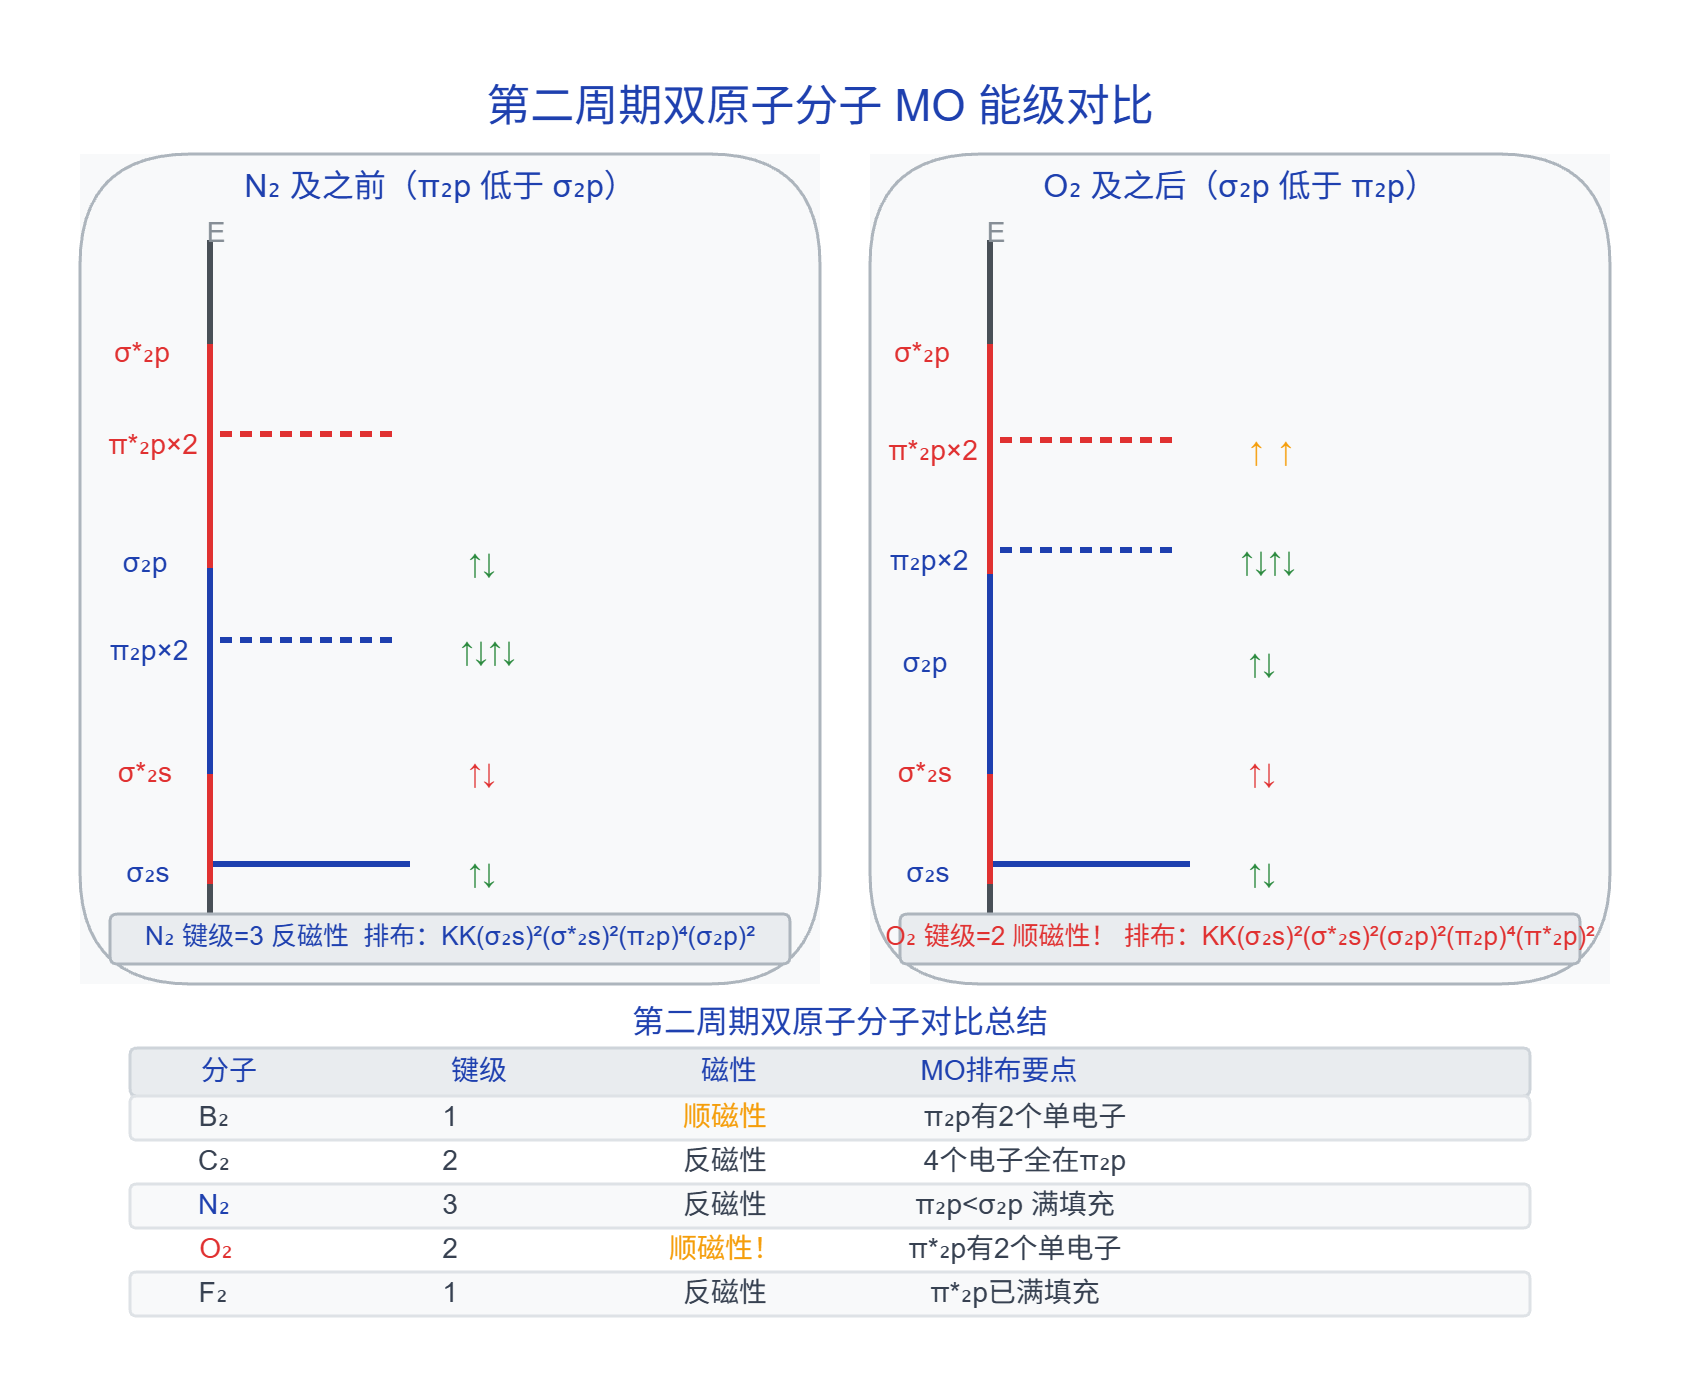
\includegraphics[width=0.45\textwidth,keepaspectratio]{media/mo-energy-diagram.jpg}
\caption{原子轨道组合成分子轨道的基本图式}
\end{figure}

\subsubsection{7.3 第二周期双原子分子 MO 能级图}\label{ux7b2cux4e8cux5468ux671fux53ccux539fux5b50ux5206ux5b50-mo-ux80fdux7ea7ux56fe}

\textbf{键级公式}：

\[
\text{键级} = \frac{\text{成键电子数} - \text{反键电子数}}{2}
\]

\textbf{两种能级顺序}：

\begin{figure}[H]\centering
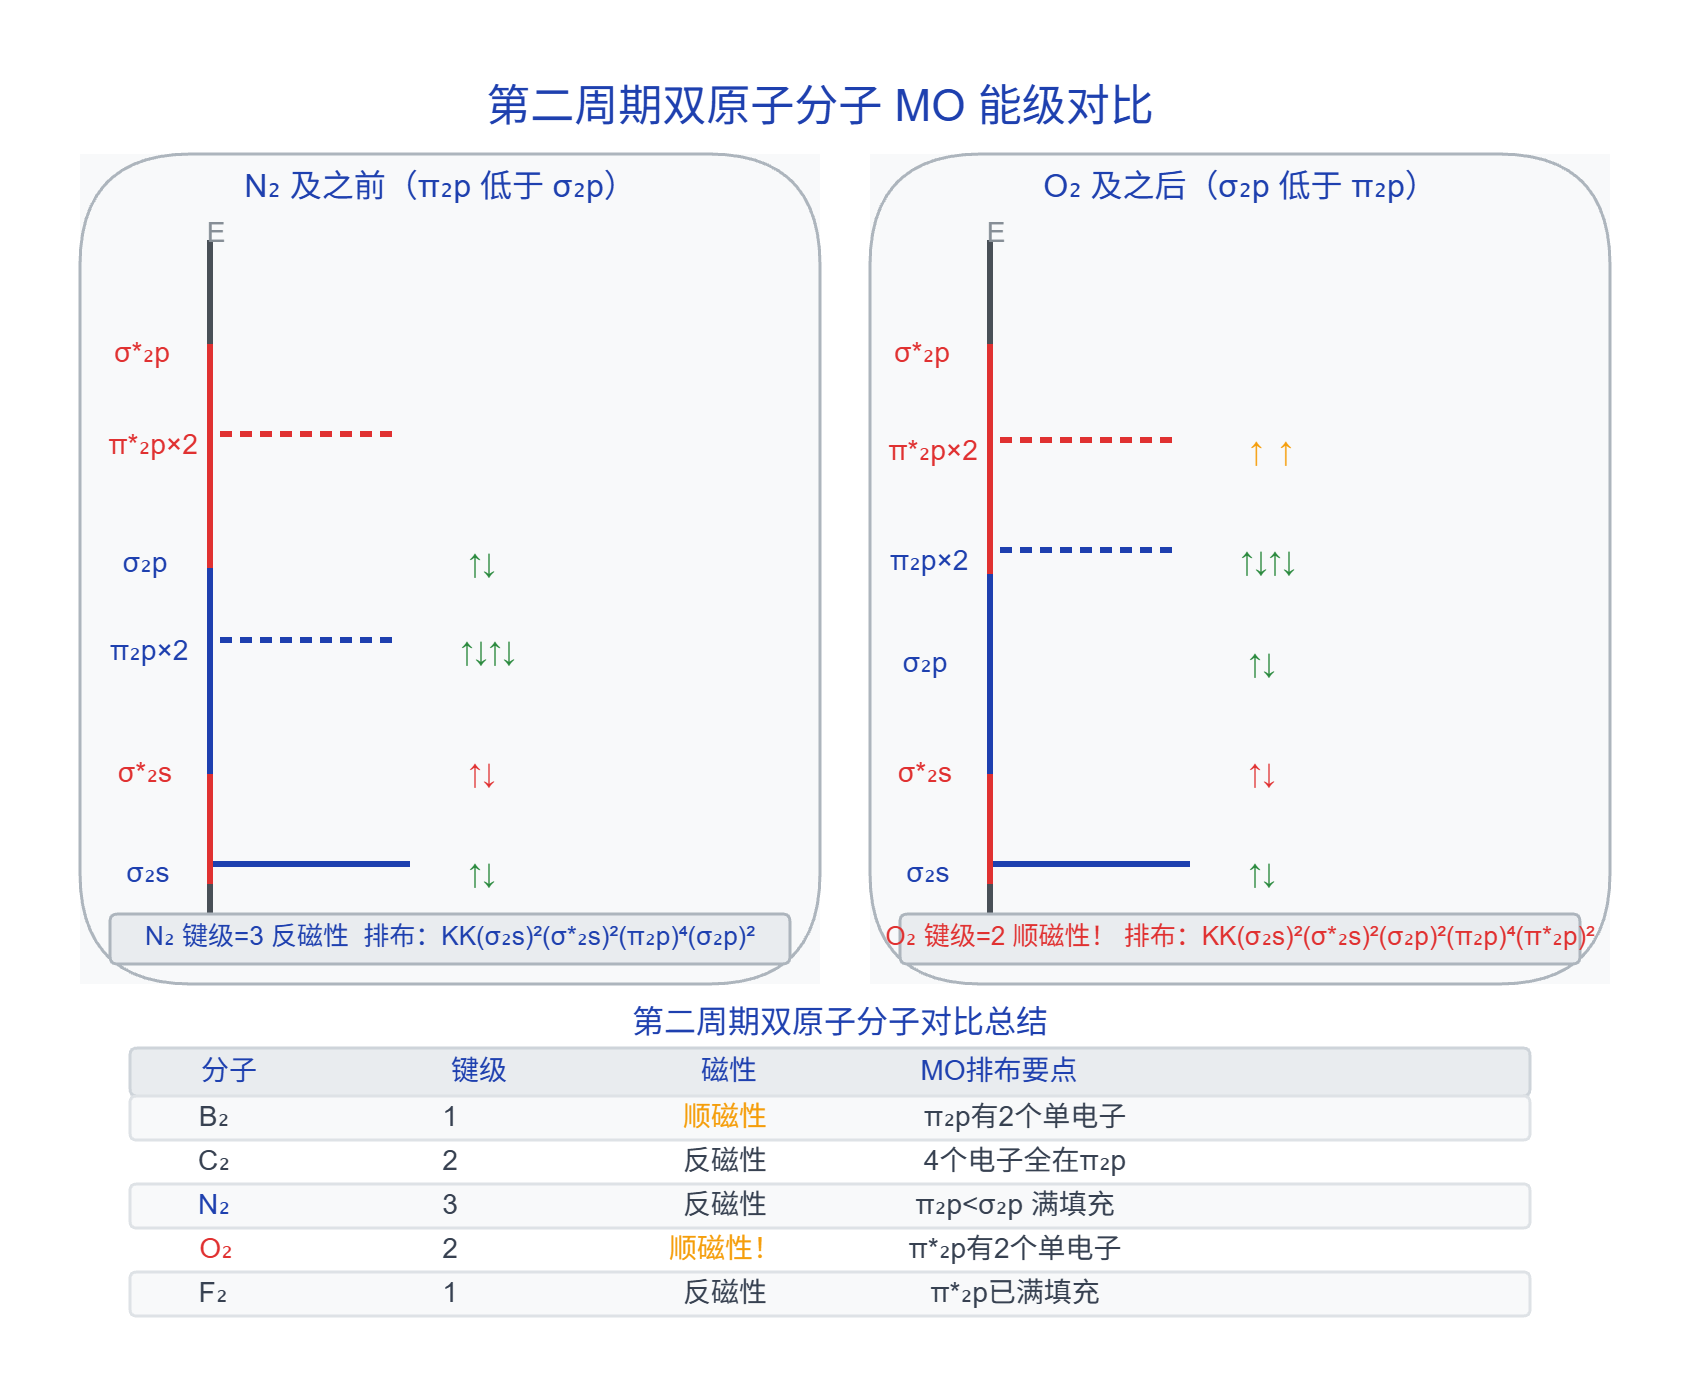
\includegraphics[width=0.45\textwidth,keepaspectratio]{media/o2-mo-diagram.jpg}
\caption{O 的分子轨道能级图}
\end{figure}

{\def\LTcaptype{none} % do not increment counter
\begin{longtable}[]{@{}lll@{}}
\toprule\noalign{}
体系 & 价层轨道顺序关键差异 & 代表分子 \\
\midrule\noalign{}
\endhead
\bottomrule\noalign{}
\endlastfoot
N\textsubscript{2} 型 & \(\pi_{2p}\) 低于 \(\sigma_{2p}\) & B\textsubscript{2}、C\textsubscript{2}、N\textsubscript{2} \\
O\textsubscript{2} 型 & \(\sigma_{2p}\) 低于 \(\pi_{2p}\) & O\textsubscript{2}、F\textsubscript{2}、Ne\textsubscript{2} \\
\end{longtable}
}

\textbf{记忆口诀}：``N\textsubscript{2} 及之前 \派\textsubscript{2}p 低于 \西格马\textsubscript{2}p，O\textsubscript{2} 及之后 \西格马\textsubscript{2}p 低于 \派\textsubscript{2}p''

\textbf{为什么有两种顺序？} 当 2s 和 2p 轨道能量差较小时(B\textsubscript{2}、C\textsubscript{2}、N\textsubscript{2})，\西格马\textsubscript{2}p 与 \派\textsubscript{2}p 发生 \textbf{sp 混杂}，\西格马\textsubscript{2}p 被推高到 \派\textsubscript{2}p 之上；当能量差较大时(O\textsubscript{2}、F\textsubscript{2})，无混杂，\西格马\textsubscript{2}p 在 \派\textsubscript{2}p 之下。

\textbf{教学洞察}：sp 混杂是 MO 理论中最容易让人困惑的概念。直观理解：当 2s 和 2p 轨道能量接近时(B、C、N 的 2s/2p 能量差小于 O、F)，\西格马\textsubscript{2}s 和 \西格马\textsubscript{2}p 会''互相排斥''---\西格马\textsubscript{2}s 被推低，\西格马\textsubscript{2}p 被推高，结果 \西格马\textsubscript{2}p 的能量高于 \派\textsubscript{2}p。这就是为什么 N\textsubscript{2} 的能级顺序特殊。\textbf{记忆口诀}：``N\textsubscript{2} 及之前 \派\textsubscript{2}p 低于 \西格马\textsubscript{2}p，O\textsubscript{2} 及之后 \西格马\textsubscript{2}p 低于 \派\textsubscript{2}p''。

\subsubsection{7.4 典型分子的 MO 电子排布}\label{ux5178ux578bux5206ux5b50ux7684-mo-ux7535ux5b50ux6392ux5e03}

{\def\LTcaptype{none} % do not increment counter
\begin{longtable}[]{@{}
  >{\centering\arraybackslash}p{(\linewidth - 8\tabcolsep) * \real{0.2083}}
  >{\centering\arraybackslash}p{(\linewidth - 8\tabcolsep) * \real{0.2083}}
  >{\raggedright\arraybackslash}p{(\linewidth - 8\tabcolsep) * \real{0.1667}}
  >{\centering\arraybackslash}p{(\linewidth - 8\tabcolsep) * \real{0.2083}}
  >{\centering\arraybackslash}p{(\linewidth - 8\tabcolsep) * \real{0.2083}}@{}}
\toprule\noalign{}
\begin{minipage}[b]{\linewidth}\centering
分子
\end{minipage} & \begin{minipage}[b]{\linewidth}\centering
价电子数
\end{minipage} & \begin{minipage}[b]{\linewidth}\raggedright
电子排布(价层)
\end{minipage} & \begin{minipage}[b]{\linewidth}\centering
键级
\end{minipage} & \begin{minipage}[b]{\linewidth}\centering
磁性
\end{minipage} \\
\midrule\noalign{}
\endhead
\bottomrule\noalign{}
\endlastfoot
B\textsubscript{2} & 6 & \(\sigma_{2s}^2 \sigma_{2s}^{*2} \pi_{2p}^2\) & 1 & 顺磁性(2 个单电子) \\
C\textsubscript{2} & 8 & \(\sigma_{2s}^2 \sigma_{2s}^{*2} \pi_{2p}^4\) & 2 & 反磁性 \\
N\textsubscript{2} & 10 & \(\sigma_{2s}^2 \sigma_{2s}^{*2} \pi_{2p}^4 \sigma_{2p}^2\) & 3 & 反磁性 \\
O\textsubscript{2} & 12 & \(\sigma_{2s}^2 \sigma_{2s}^{*2} \sigma_{2p}^2 \pi_{2p}^4 \pi_{2p}^{*2}\) & 2 & \textbf{顺磁性}(2 个单电子){[}完成{]} \\
F\textsubscript{2} & 14 & \(\sigma_{2s}^2 \sigma_{2s}^{*2} \sigma_{2p}^2 \pi_{2p}^4 \pi_{2p}^{*4}\) & 1 & 反磁性 \\
Ne\textsubscript{2} & 16 & 满填 & 0 & 不存在 \\
\end{longtable}
}

相关 KP：分子轨道理论、键级

\textbf{练习：第二周期双原子分子 MO 信息补全}

{\def\LTcaptype{none} % do not increment counter
\begin{longtable}[]{@{}cclcc@{}}
\toprule\noalign{}
分子/离子 & 价电子数 & 电子排布(价层) & 键级 & 磁性 \\
\midrule\noalign{}
\endhead
\bottomrule\noalign{}
\endlastfoot
B\textsubscript{2} & 6 & \(\sigma_{2s}^2 \sigma_{2s}^{*2} \pi_{2p}^2\) & 1 & 顺磁性 \\
C\textsubscript{2} & 8 & \_\_\_\_ & \_\_\_\_ & \_\_\_\_ \\
N\textsubscript{2} & 10 & \_\_\_\_ & \_\_\_\_ & \_\_\_\_ \\
O\textsubscript{2} & 12 & \_\_\_\_ & \_\_\_\_ & \_\_\_\_ \\
O\textsubscript{2}\textsuperscript{-} & 13 & \_\_\_\_ & \_\_\_\_ & \_\_\_\_ \\
O\textsubscript{2}\textsuperscript{2-} & 14 & \_\_\_\_ & \_\_\_\_ & \_\_\_\_ \\
F\textsubscript{2} & 14 & \_\_\_\_ & \_\_\_\_ & \_\_\_\_ \\
\end{longtable}
}

提示：注意 N\textsubscript{2} 和 O\textsubscript{2} 的能级顺序不同。O\textsubscript{2} 体系用 O\textsubscript{2} 型顺序(\(\sigma_{2p}<\pi_{2p}\))，O\textsubscript{2}\textsuperscript{2-} 有 14 个价电子，会填满 \(\pi_{2p}^*\)。

\begin{center}\rule{0.5\linewidth}{0.5pt}\end{center}

\subsection{八、分子间作用力 --- 从分子到聚集态}\label{ux516bux5206ux5b50ux95f4ux4f5cux7528ux529b-ux4eceux5206ux5b50ux5230ux805aux96c6ux6001}

前面六节都在讨论\textbf{单个分子内部}的结构和成键。但化学世界是由大量分子聚集而成的---水为什么是液体(而不是气体)？蜡为什么是固体？为什么 NH\textsubscript{3} 在水中溶解度极大而 PH\textsubscript{3} 极小？

答案就在\textbf{分子之间}的作用力。虽然这些力比化学键弱得多(1--40 kJ/mol 对比 100--800 kJ/mol)，但它们决定了物质的\textbf{熔点、沸点、溶解度、表面张力}等一切宏观物理性质。

\textbf{为何重要}：分子间力是连接''微观分子结构''与''宏观物理性质''的桥梁。竞赛中约 30\% 的结构化学简答题最终落脚到分子间力解释---比如''为什么 H\textsubscript{2}O 的沸点高于 H\textsubscript{2}S''\,``为什么 NH\textsubscript{3} 在水中溶解度极大''。

\subsubsection{8.1 分子间力概述}\label{ux5206ux5b50ux95f4ux529bux6982ux8ff0}

分子间作用力虽然弱于化学键(\textasciitilde1--40 kJ/mol vs 100--800 kJ/mol)，但决定物质的\textbf{熔点、沸点、溶解度}等物理性质。

{\def\LTcaptype{none} % do not increment counter
\begin{longtable}[]{@{}llcll@{}}
\toprule\noalign{}
类型 & 本质 & 强度 & 存在范围 & 实例 \\
\midrule\noalign{}
\endhead
\bottomrule\noalign{}
\endlastfoot
\textbf{色散力} & 瞬时偶极 & 最弱 & 所有分子/原子 & 稀有气体液化 \\
\textbf{诱导力} & 永久偶极诱导 & 较弱 & 极性+非极性 & O\textsubscript{2} 溶于水 \\
\textbf{取向力} & 永久偶极间 & 较强 & 极性分子间 & HCl、H\textsubscript{2}O \\
\end{longtable}
}

记忆口诀：\textbf{``极性有取向，极化生诱导，万物有色散''}

\begin{figure}[H]\centering
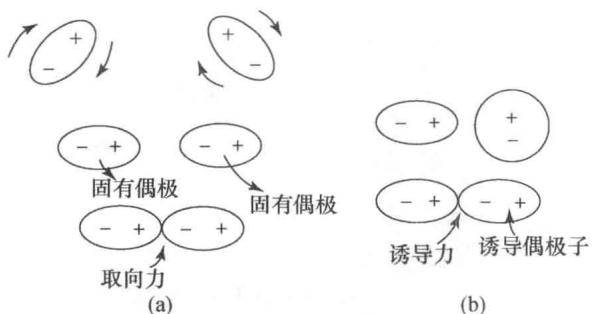
\includegraphics[width=0.45\textwidth,keepaspectratio]{media/12-26-orientation-induction-intermolecular-forces.jpg}
\hspace{0.02\textwidth}
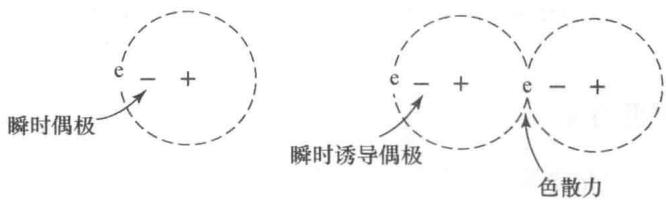
\includegraphics[width=0.45\textwidth,keepaspectratio]{media/12-27-dispersion-force-nonpolar-molecules.jpg}
\caption{取向力、诱导力与色散力示意}
\end{figure}

\subsubsection{8.2 氢键}\label{ux6c22ux952e}

\textbf{形成条件}(缺一不可)：
1. 有 X-H 键(X = F、O、N)
2. Y 上有孤对电子(Y = F、O、N)
3. X、Y 电负性大、半径小

\textbf{教学洞察}：氢键的本质是一种\textbf{特殊的偶极-偶极相互作用}，强度介于化学键和范德华力之间。学生最常问的问题是---``为什么 NH\textsubscript{3} 的沸点比 H\textsubscript{2}O 低？NH\textsubscript{3} 也能形成氢键啊！''答案是：\textbf{每个 H\textsubscript{2}O 可以形成 4 个氢键(2 个 O-H 供体 + 2 对孤对受体)，而 NH\textsubscript{3} 只能形成 2 个(3 个 N-H 供体但只有 1 对孤对受体)}。水中的氢键网络更加立体和完整，因此破坏它需要更多能量。

\textbf{易错提醒}：氢键的\textbf{方向性}(X-H···Y 趋向于 180°)和\textbf{饱和性}(每个 X-H 只能与一个 Y 形成氢键)经常被忽视。判断一个分子能否形成氢键时，记住：\textbf{必须同时有 X-H(供体)和 Y 上的孤对电子(受体)}---CH\textsubscript{4} 虽然有 C-H 键，但 C 的电负性太小(2.5)，不能形成氢键。

\textbf{氢键强度序列}：

\[
\text{F-H} \cdots \text{F} > \text{O-H} \cdots \text{O} > \text{O-H} \cdots \text{N} > \text{N-H} \cdots \text{O} > \text{N-H} \cdots \text{N}
\]

\textbf{氢键的特点}：
- \textbf{方向性}：X-H···Y 趋向于直线排列(\textasciitilde180°)
- \textbf{饱和性}：每个 X-H 只能与一个 Y 形成氢键

\textbf{氢键对物性的影响}：

{\def\LTcaptype{none} % do not increment counter
\begin{longtable}[]{@{}lll@{}}
\toprule\noalign{}
性质 & 效应 & 经典例证 \\
\midrule\noalign{}
\endhead
\bottomrule\noalign{}
\endlastfoot
沸点 & 含氢键的分子沸点大幅升高 & H\textsubscript{2}O(100°C) vs H\textsubscript{2}S(-60°C) \\
溶解度 & 溶质与溶剂形成氢键\箭溶解度增大 & NH\textsubscript{3} 在水中溶解度极大 \\
密度 & 冰中氢键形成空旷结构\箭密度小于水 & 冰浮于水上 \\
\end{longtable}
}

相关 KP：分子间力、氢键、范德华力

\begin{center}\rule{0.5\linewidth}{0.5pt}\end{center}

\subsection{九、典型例题}\label{ux4e5dux5178ux578bux4f8bux9898}

\textbf{题目}：画出 XeF\textsubscript{2} 的 Lewis 结构，标出形式电荷，判断中心原子的杂化方式与分子构型。

\textbf{题目}：比较 (CH\textsubscript{3})\textsubscript{3}N 和 (SiH\textsubscript{3})\textsubscript{3}N 的分子构型，解释差异的原因。

\textbf{题目}：用分子轨道理论比较 N\textsubscript{2}、O\textsubscript{2}、O\textsubscript{2}\textsuperscript{-} 的键级与磁性。

\textbf{题目}：解释以下实验现象：
(1) H\textsubscript{2}O 的沸点(100°C)远高于 H\textsubscript{2}S(-60°C)
(2) NH\textsubscript{3} 在水中的溶解度极大，而 PH\textsubscript{3} 溶解度很小

\textbf{题目}：SO\textsubscript{2} 是一种常见的 V 形分子，已知其 S-O 键长(143 pm)介于 S-O 单键(\textasciitilde157 pm)和 S=O 双键(\textasciitilde122 pm)之间。

\begin{enumerate}
\def\labelenumi{(\arabic{enumi})}
\tightlist
\item
  画出 SO\textsubscript{2} 的 Lewis 结构(考虑形式电荷)，写出可能的共振结构。
\item
  用 VSEPR 理论预测 SO\textsubscript{2} 的分子构型和键角。
\item
  判断 S 的杂化方式。
\item
  SO\textsubscript{2} 中是否存在离域\派键？若存在，写出 \派ₙᵐ 表示并分析电子来源。
\item
  根据以上分析解释为什么 S-O 键长介于单键和双键之间。
\end{enumerate}

\textbf{题目}：CO 是初赛高频考点。它与 N\textsubscript{2} 等电子(若按价电子计均为 10，若按总电子数计均为 14)，但 CO 与过渡金属的配位能力远强于 N\textsubscript{2}。

\begin{enumerate}
\def\labelenumi{(\arabic{enumi})}
\tightlist
\item
  画出 CO 的 MO 能级图(参照 N\textsubscript{2} 的能级顺序，因 s-p 混杂显著)。
\item
  计算 CO 的键级并判断磁性。
\item
  写出 CO 的 Lewis 结构。它含有几个配位键？
\item
  用 MO 理论解释：为什么 CO 的配位能力强于 N\textsubscript{2}？
\end{enumerate}

\textbf{题目}：一未知离子 X 的化学式为 NCO\textsuperscript{-}(氰酸根离子)，已知它有三种可能的共振结构。

\begin{enumerate}
\def\labelenumi{(\arabic{enumi})}
\tightlist
\item
  画出 NCO\textsuperscript{-} 中所有可能满足八隅体规则的共振结构(N 为端基原子，C 为中心原子)，标出形式电荷，选出最优结构。
\item
  用 VSEPR 理论预测 NCO\textsuperscript{-} 的分子构型，判断中心 C 的杂化方式。
\item
  判断 NCO\textsuperscript{-} 与哪些分子/离子等电子，写出 2-3 个等电子体。
\item
  若将 NCO\textsuperscript{-} 中的 N 换为 S(得到 SCO)，SCO 的构型是否与 NCO\textsuperscript{-} 相同？键角会如何变化？
\end{enumerate}

\begin{center}\rule{0.5\linewidth}{0.5pt}\end{center}

\textbf{例题答案}

\textbf{例1}：XeF\textsubscript{2} 总价电子数为 22。Lewis 结构可写作 F-Xe-F，Xe 上有 3 对孤对、每个 F 上有 3 对孤对，形式电荷均为 0；AX\textsubscript{2}E\textsubscript{3}，分子为直线形，中心 Xe 常用 sp\textsuperscript{3}d 描述。

\textbf{例2}：(CH\textsubscript{3})\textsubscript{3}N 中 N 的孤对保留在杂化轨道里，分子呈三角锥形，N 为 sp\textsuperscript{3} 杂化；(SiH\textsubscript{3})\textsubscript{3}N 中孤对可向 Si 的低能空轨道离域，N 更接近平面三角形，常用 sp\textsuperscript{2} 杂化描述。

\textbf{例3}：N\textsubscript{2} 的键级为 3、反磁性；O\textsubscript{2} 的键级为 2、顺磁性；O\textsubscript{2}\textsuperscript{-} 的键级为 1.5、顺磁性。稳定性顺序可记为 N\textsubscript{2} \textgreater{} O\textsubscript{2} \textgreater{} O\textsubscript{2}\textsuperscript{-}。

\textbf{例4}：H\textsubscript{2}O 分子间存在氢键，H\textsubscript{2}S 仅有较弱范德华力，所以 H\textsubscript{2}O 沸点显著更高；NH\textsubscript{3} 与 H\textsubscript{2}O 之间可形成氢键，而 PH\textsubscript{3} 基本不能形成有效氢键，因此 NH\textsubscript{3} 在水中的溶解度远大于 PH\textsubscript{3}。

\textbf{例5}：SO\textsubscript{2} 总价电子数为 18，主要共振式可写成 O=S-O\textsuperscript{-} 与 \textsuperscript{-}O-S=O。中心 S 周围共有 3 个电子对区域，因此构型为 AX\textsubscript{2}E、分子呈 V 形，键角略小于 120°，S 近似 sp\textsuperscript{2} 杂化；体系中可用 \派\textsubscript{3}\textsuperscript{4} 描述离域\派键，平均键级约为 1.5，所以 S-O 键长介于单键和双键之间。

\textbf{例6}：CO 与 N\textsubscript{2} 若按价电子计都为 10 个，若按总电子数计都为 14 个。CO 的价层 MO 排布与 N\textsubscript{2} 型相似，键级为 3、反磁性；Lewis 结构常写作 \(\mathrm{:C\equiv O:}\)，也可把其中一条键看作 O\箭C 的配位键。它比 N\textsubscript{2} 更易与金属配位，关键在于 C 端 HOMO 系数更大、\西格马 给予更强，同时 \派* 轨道便于接受金属 d 电子反馈。

\textbf{例7}：NCO\textsuperscript{-} 总价电子数为 16，骨架为 N-C-O，中心 C 为 sp 杂化，整体呈直线形。主要共振式以 N≡C-O\textsuperscript{-} 为主，\textsuperscript{-}N=C=O 也是重要贡献式；可与 CO\textsubscript{2}、NO\textsubscript{2}\textsuperscript{+}、SCN\textsuperscript{-} 等一起按``16 电子 + 3 原子''做等电子迁移。若把 N 换成 S 得到 SCO，构型仍为直线形，但 S-C 键更长、极性分布也会改变。

\subsection{十、方法总结 · 结构预测工具链}\label{ux5341ux65b9ux6cd5ux603bux7ed3-ux7ed3ux6784ux9884ux6d4bux5de5ux5177ux94fe}

\subsubsection{10.1 使用顺序}\label{ux4f7fux7528ux987aux5e8f}

\begin{enumerate}
\def\labelenumi{\arabic{enumi}.}
\setcounter{enumi}{-1}
\tightlist
\item
  先判断化学键类型(离子/共价/金属)，用电负性差 Δχ 快速分类。
\item
  再用 Lewis 结构定总价电子数、骨架和形式电荷。
\item
  再用 VSEPR 判断电子对几何与实际分子构型。
\item
  再看 \西格马 键数 + 孤对数，反推中心原子的杂化方式。
\item
  再检查是否存在离域\派键，必要时用等电子体快速迁移结构。
\item
  最后在键级、磁性和物性问题上调用 MO 理论与分子间力分析。
\end{enumerate}

\subsubsection{10.2 核心速查表}\label{ux6838ux5fc3ux901fux67e5ux8868}

{\def\LTcaptype{none} % do not increment counter
\begin{longtable}[]{@{}
  >{\raggedright\arraybackslash}p{(\linewidth - 6\tabcolsep) * \real{0.2500}}
  >{\raggedright\arraybackslash}p{(\linewidth - 6\tabcolsep) * \real{0.2500}}
  >{\raggedright\arraybackslash}p{(\linewidth - 6\tabcolsep) * \real{0.2500}}
  >{\raggedright\arraybackslash}p{(\linewidth - 6\tabcolsep) * \real{0.2500}}@{}}
\toprule\noalign{}
\begin{minipage}[b]{\linewidth}\raggedright
工具
\end{minipage} & \begin{minipage}[b]{\linewidth}\raggedright
核心公式/规律
\end{minipage} & \begin{minipage}[b]{\linewidth}\raggedright
适用场景
\end{minipage} & \begin{minipage}[b]{\linewidth}\raggedright
常见陷阱
\end{minipage} \\
\midrule\noalign{}
\endhead
\bottomrule\noalign{}
\endlastfoot
\textbf{化学键分类} & Δχ \textless{} 0.4 非极性，0.4\textasciitilde1.9 极性，\textgreater{} 1.9 离子 & 快速判断键型 & HF(Δχ=1.9) 是共价键---阈值有灰区 \\
\textbf{Lewis 结构} & 五步法；FC = 价电子 - 孤对 - ½成键 & 判断成键方式和电子分布 & 形式电荷 \不等于 实际电荷 \\
\textbf{VSEPR} & AXₙEₘ；孤对-孤对 \textgreater{} 孤对-成键 \textgreater{} 成键-成键 & 预测分子构型 & 多重键视为 1 个区域 \\
\textbf{杂化轨道} & \西格马 键数 + 孤对轨道数 \箭 杂化类型 & 解释键角和构型 & 杂化发生在成键过程中 \\
**离域\派键** & \派ₙᵐ：共面 + 平行 p 轨道 + m \textless{} 2n & 分析共轭体系 & 电子计数错误(常见漏计或重计) \\
\textbf{等电子体} & 同价电子数 + 同原子数 \箭 同结构 & 推断未知物种 & 忘了必须同时满足两个条件 \\
\textbf{MO 理论} & 键级 = (成键-反键)/2 & 判断键级、磁性 & B\textsubscript{2}-N\textsubscript{2} 与 O\textsubscript{2}-F\textsubscript{2} 能级顺序不同 \\
\textbf{分子间力} & 取向力(极性)+ 诱导力(极化)+ 色散力(所有) & 解释物性 & 氢键与范德华力混淆 \\
\end{longtable}
}

\begin{center}\rule{0.5\linewidth}{0.5pt}\end{center}

\subsection{十一、练习题}\label{ux5341ux4e00ux7ec3ux4e60ux9898}

\textbf{化学键与电负性}

\begin{enumerate}
\def\labelenumi{\arabic{enumi}.}
\item
  判断下列各对原子间化学键的类型(离子键/极性共价键/非极性共价键)：Na-Cl、H-H、H-O、C-F、Cs-F。
\item
  按电负性从大到小排列以下元素：O、C、Na、F、Cl、N，并指出哪些元素间可形成离子键。
\end{enumerate}

\textbf{\西格马 键与 \派 键}

\begin{enumerate}
\def\labelenumi{\arabic{enumi}.}
\setcounter{enumi}{2}
\item
  指出下列分子中 \西格马 键和 \派 键的数目：CO\textsubscript{2}、HCN、C\textsubscript{2}H\textsubscript{2}(乙炔)、CH\textsubscript{2}=CH\textsubscript{2}(乙烯)。
\item
  为什么 H\textsubscript{2}O 中 O-H 键可以自由旋转而 C=C 双键不可以？用 \西格马/\派 键概念解释。
\end{enumerate}

\textbf{Lewis 结构与形式电荷}

\begin{enumerate}
\def\labelenumi{\arabic{enumi}.}
\setcounter{enumi}{4}
\item
  画出下列分子/离子的 Lewis 结构，标出形式电荷：CO\textsubscript{2}、SO\textsubscript{2}、ClO\textsubscript{4}\textsuperscript{-}、BrF\textsubscript{3}、XeF\textsubscript{2}。
\item
  判断下列 Lewis 结构中哪个更稳定(形式电荷更接近零)：(a) SO\textsubscript{2} 的两种共振式；(b) CO 的两种共振式(C≡O 和 C=O)。
\end{enumerate}

\textbf{VSEPR 与杂化}

\begin{enumerate}
\def\labelenumi{\arabic{enumi}.}
\setcounter{enumi}{6}
\item
  用 VSEPR 理论判断下列分子的空间构型：PCl\textsubscript{5}、SF\textsubscript{4}、ClF\textsubscript{3}、IF\textsubscript{4}\textsuperscript{-}、BrF\textsubscript{5}、XeF\textsubscript{4}。
\item
  判断下列分子的中心原子杂化类型及是否有孤对电子：CO\textsubscript{2}、BF\textsubscript{3}、CH\textsubscript{4}、PCl\textsubscript{5}、SF\textsubscript{6}、H\textsubscript{2}O、NH\textsubscript{3}、XeF\textsubscript{2}。
\item
  为什么 H\textsubscript{2}O 的键角(104.5°)小于 NH\textsubscript{3}(107°)？用杂化理论和 VSEPR 解释。
\end{enumerate}

**离域\派键与等电子体**

\begin{enumerate}
\def\labelenumi{\arabic{enumi}.}
\setcounter{enumi}{9}
\item
  写出下列分子/离子中的离域\派键类型(\派ₙᵐ)：NO\textsubscript{3}\textsuperscript{-}、CO\textsubscript{3}\textsuperscript{2-}、SO\textsubscript{2}、O\textsubscript{3}、苯 C\textsubscript{6}H\textsubscript{6}。
\item
  用等电子体原理推断 N\textsubscript{3}\textsuperscript{-}、NO\textsubscript{2}\textsuperscript{+}、SCN\textsuperscript{-}、ClO\textsubscript{4}\textsuperscript{-} 的空间构型。
\end{enumerate}

\textbf{分子间力}

\begin{enumerate}
\def\labelenumi{\arabic{enumi}.}
\setcounter{enumi}{11}
\item
  按沸点从高到低排列：H\textsubscript{2}O、H\textsubscript{2}S、H\textsubscript{2}Se、H\textsubscript{2}Te，并解释趋势中的反常。
\item
  解释为什么 NH\textsubscript{3} 在水中溶解度极大而 PH\textsubscript{3} 溶解度极小。
\item
  画出 HF 分子间氢键的示意图，标出氢键供体和受体。
\end{enumerate}

\textbf{MO 理论深入}

\begin{enumerate}
\def\labelenumi{\arabic{enumi}.}
\setcounter{enumi}{14}
\item
  画出 N\textsubscript{2}、O\textsubscript{2}、F\textsubscript{2} 的 MO 能级图，计算键级，判断磁性。注意 N\textsubscript{2} 和 O\textsubscript{2} 的能级顺序差异。
\item
  已知 B\textsubscript{2} 分子具有顺磁性。用 MO 理论解释这一现象，计算 B\textsubscript{2} 的键级，并与 C\textsubscript{2} 比较。
\item
  画出 CO 的 MO 能级图(异核双原子分子)，计算键级。解释为什么 CO 的偶极矩(0.12 D)比预期小得多。
\end{enumerate}

\textbf{结构综合分析}

\begin{enumerate}
\def\labelenumi{\arabic{enumi}.}
\setcounter{enumi}{17}
\item
  比较 CO 和 N\textsubscript{2} 的结构：(a) 二者是等电子体，MO 能级图相似；(b) CO 的偶极矩方向是 C\textsuperscript{-}-O\textsuperscript{+}，解释原因；(c) CO 与过渡金属的配位能力远强于 N\textsubscript{2}，从 \西格马-给予/\派-反馈角度解释。
\item
  某分子 X 的分子式为 AB\textsubscript{2}，中心原子 A 有 2 对孤对电子。若 A 在第二周期，X 可能是什么？若 A 在第三周期呢？
\item
  用 MO 理论解释 O\textsubscript{2} 的顺磁性，并说明为什么 O\textsubscript{2}\textsuperscript{-}(超氧离子)和 O\textsubscript{2}\textsuperscript{2-}(过氧离子)的键级分别降低。
\end{enumerate}

\textbf{氢键与特殊分子间力}

\begin{enumerate}
\def\labelenumi{\arabic{enumi}.}
\setcounter{enumi}{20}
\item
  解释以下''反常''现象：(a) HF 的沸点(19.5°C)远高于 HCl(-85°C)；(b) 冰的密度小于液态水。
\item
  乙醇(CH\textsubscript{3}CH\textsubscript{2}OH)和二甲醚(CH\textsubscript{3}OCH\textsubscript{3})是同分异构体，但沸点差异巨大(78°C vs -24°C)。解释原因。
\item
  \textbf{(改编自全国初赛)} IF\textsubscript{7} 是已知的稳定分子，I 的配位数达到 7。

  \begin{enumerate}
  \def\labelenumii{(\alph{enumii})}
  \tightlist
  \item
    画出 IF\textsubscript{7} 的 Lewis 结构，判断中心 I 是否满足八隅体规则。
  \item
    用 VSEPR 理论预测 IF\textsubscript{7} 的几何构型。
  \item
    判断 I 的杂化类型。
  \item
    第七周期元素能否形成类似 MF\textsubscript{7} 的分子？为什么？
  \end{enumerate}
\item
  \textbf{(共轭体系综合题)} 1,3-丁二烯(CH\textsubscript{2}=CH-CH=CH\textsubscript{2})：

  \begin{enumerate}
  \def\labelenumii{(\alph{enumii})}
  \tightlist
  \item
    每个 C 的杂化方式？分子是否共平面？
  \item
    指出离域\派键类型(\派ₙᵐ)，画出电子离域示意图。
  \item
    C2-C3 单键键长(147 pm)比乙烷的 C-C(154 pm)短，解释原因。
  \item
    1,3-丁二烯的 \派\textsubscript{4}\textsuperscript{4} 离域与苯的 \派\textsubscript{6}\textsuperscript{6} 离域有何本质区别？
  \end{enumerate}
\item
  \textbf{(CO 与过渡金属成键)} CO 是重要的\派酸配体。

  \begin{enumerate}
  \def\labelenumii{(\alph{enumii})}
  \tightlist
  \item
    画出 CO 的 MO 能级图，标出最高占据轨道和最低空轨道。
  \item
    解释 CO 的 C 端而非 O 端与金属配位的原因。
  \item
    在金属羰基化合物 M(CO)\textsubscript{6} 中，M\箭CO 的\派反馈键如何影响 C-O 键长和红外吸收频率？
  \end{enumerate}
\item
  \textbf{(综合推断题)} 某未知分子 X 满足以下条件：

  \begin{itemize}
  \tightlist
  \item
    含一个第二周期中心原子 A 和两个相同配体 B
  \item
    A 的氧化态为 +4
  \item
    分子具有顺磁性
  \item
    总价电子数为 18
  \end{itemize}

  \begin{enumerate}
  \def\labelenumii{(\alph{enumii})}
  \tightlist
  \item
    推断 X 的可能化学式。
  \item
    画出 Lewis 结构和 MO 能级图。
  \item
    解释其顺磁性的来源。
  \end{enumerate}
\item
  \textbf{(超价分子分析)} XeO\textsubscript{3} 和 XeO\textsubscript{4} 都是已知的氙氧化物。

  \begin{enumerate}
  \def\labelenumii{(\alph{enumii})}
  \tightlist
  \item
    分别画出二者的 Lewis 结构。
  \item
    用 VSEPR 预测几何构型。
  \item
    XeO\textsubscript{3} 和 XeO\textsubscript{4} 的稳定性差异如何解释？
  \item
    为什么 Xe 能形成这些化合物而 Ne 不能？
  \end{enumerate}
\end{enumerate}

\begin{center}\rule{0.5\linewidth}{0.5pt}\end{center}

\subsection{十二、参考答案与提示}\label{ux5341ux4e8cux53c2ux8003ux7b54ux6848ux4e0eux63d0ux793a}

\textbf{§一 化学键基础练习}：

\begin{enumerate}
\def\labelenumi{\arabic{enumi}.}
\item
  Na-Cl：离子键(Δχ = 2.1)；H-H：非极性共价键(Δχ = 0)；H-O：极性共价键(Δχ = 1.4)；C-F：极性共价键(Δχ = 1.5)；Cs-F：离子键(Δχ = 3.3)。
\item
  电负性排序：F(4.0) \textgreater{} O(3.5) \textgreater{} N(3.0) \textgreater{} Cl(3.0) \textgreater{} C(2.5) \textgreater{} Na(0.9)。Na 与 F、O、Cl、N 之间均可形成离子键(Δχ \textgreater{} 1.9)。
\item
  CO\textsubscript{2}：2 个 \西格马 键 + 2 个 \派 键(2 个 C=O 双键，每个含 1\西格马 + 1\派)；HCN：2 个 \西格马 键 + 2 个 \派 键(C-H 为 \西格马，C≡N 含 1\西格马 + 2\派)；C\textsubscript{2}H\textsubscript{2}：3 个 \西格马 键 + 2 个 \派 键(2 个 C-H \西格马 + 1 个 C-C \西格马，C≡C 含 2\派)；CH\textsubscript{2}=CH\textsubscript{2}：5 个 \西格马 键 + 1 个 \派 键(4 个 C-H \西格马 + 1 个 C-C \西格马，C=C 含 1\派)。
\item
  H\textsubscript{2}O 中 O-H 键为 \西格马 键，\西格马 键可绕键轴自由旋转；C=C 双键含 1 个 \派 键，\派 键的电子云分布在键轴上下两侧，旋转会破坏 \派 键重叠\箭不可旋转。
\end{enumerate}

\textbf{§二 Lewis 结构练习}(五步法)：

{\def\LTcaptype{none} % do not increment counter
\begin{longtable}[]{@{}
  >{\centering\arraybackslash}p{(\linewidth - 6\tabcolsep) * \real{0.2632}}
  >{\centering\arraybackslash}p{(\linewidth - 6\tabcolsep) * \real{0.2632}}
  >{\centering\arraybackslash}p{(\linewidth - 6\tabcolsep) * \real{0.2632}}
  >{\raggedright\arraybackslash}p{(\linewidth - 6\tabcolsep) * \real{0.2105}}@{}}
\toprule\noalign{}
\begin{minipage}[b]{\linewidth}\centering
分子/离子
\end{minipage} & \begin{minipage}[b]{\linewidth}\centering
S
\end{minipage} & \begin{minipage}[b]{\linewidth}\centering
中心八隅体？
\end{minipage} & \begin{minipage}[b]{\linewidth}\raggedright
孤对
\end{minipage} \\
\midrule\noalign{}
\endhead
\bottomrule\noalign{}
\endlastfoot
SO\textsubscript{2} & 18 & \href{3\%20个电子对区域}{完成} & S 有 1 对，每个 O 有 2 对(调整后) \\
ClO\textsubscript{4}\textsuperscript{-} & 32 & {[}完成{]} & 每个 O 有 3 对孤对 \\
BrF\textsubscript{3} & 28 & \href{5\%20个电子对区域}{完成} & Br 有 2 对孤对，F 各有 3 对 \\
\end{longtable}
}

\textbf{§三 VSEPR 分类练习}：

{\def\LTcaptype{none} % do not increment counter
\begin{longtable}[]{@{}ccccll@{}}
\toprule\noalign{}
分子 & n & m & AXₙEₘ & 理想排布 & 实际构型 \\
\midrule\noalign{}
\endhead
\bottomrule\noalign{}
\endlastfoot
ClF\textsubscript{3} & 3 & 2 & AX\textsubscript{3}E\textsubscript{2} & 三角双锥 & T 形 \\
XeF\textsubscript{2} & 2 & 3 & AX\textsubscript{2}E\textsubscript{3} & 三角双锥 & 直线形 \\
IF\textsubscript{4}\textsuperscript{-} & 4 & 2 & AX\textsubscript{4}E\textsubscript{2} & 八面体 & 平面正方形 \\
\end{longtable}
}

\textbf{§四 杂化类型练习}：

{\def\LTcaptype{none} % do not increment counter
\begin{longtable}[]{@{}ccccc@{}}
\toprule\noalign{}
分子 & \西格马 键数 & 孤对 & 总数 & 杂化 \\
\midrule\noalign{}
\endhead
\bottomrule\noalign{}
\endlastfoot
BF\textsubscript{3} & 3 & 0 & 3 & sp\textsuperscript{2} \\
H\textsubscript{2}O & 2 & 2 & 4 & sp\textsuperscript{3}(不等性) \\
SF\textsubscript{6} & 6 & 0 & 6 & sp\textsuperscript{3}d\textsuperscript{2} \\
PCl\textsubscript{5} & 5 & 0 & 5 & sp\textsuperscript{3}d \\
XeF\textsubscript{2} & 2 & 3 & 5 & sp\textsuperscript{3}d \\
\end{longtable}
}

\textbf{§五 \派ₙᵐ 计数练习}：

{\def\LTcaptype{none} % do not increment counter
\begin{longtable}[]{@{}cclccc@{}}
\toprule\noalign{}
分子/离子 & n & 各原子 p 电子数 & 电荷调整 & m & \派ₙᵐ \\
\midrule\noalign{}
\endhead
\bottomrule\noalign{}
\endlastfoot
CO\textsubscript{3}\textsuperscript{2-} & 4 & C:1, O:1+1+1 & +2(负电荷) & 6 & \派\textsubscript{4}\textsuperscript{6} \\
SO\textsubscript{2} & 3 & S:2, O:1+1 & 0 & 4 & \派\textsubscript{3}\textsuperscript{4} \\
O\textsubscript{3} & 3 & 中心 O:2, 两端 O:1+1 & 0 & 4 & \派\textsubscript{3}\textsuperscript{4} \\
苯 C\textsubscript{6}H\textsubscript{6} & 6 & 每个 C:1 & 0 & 6 & \派\textsubscript{6}\textsuperscript{6} \\
\end{longtable}
}

\textbf{§六 等电子体练习}：

{\def\LTcaptype{none} % do not increment counter
\begin{longtable}[]{@{}cccll@{}}
\toprule\noalign{}
物种 & 价电子数 & 原子数 & 等电子体 & 构型 \\
\midrule\noalign{}
\endhead
\bottomrule\noalign{}
\endlastfoot
O\textsubscript{3} & 18 & 3 & SO\textsubscript{2} & V 形 \\
SCN\textsuperscript{-} & 16 & 3 & CO\textsubscript{2} & 直线形 \\
NO\textsubscript{2}\textsuperscript{+} & 16 & 3 & CO\textsubscript{2} & 直线形 \\
ClO\textsubscript{4}\textsuperscript{-} & 32 & 5 & PO\textsubscript{4}\textsuperscript{3-}、SO\textsubscript{4}\textsuperscript{2-} & 四面体 \\
\end{longtable}
}

\textbf{§七 MO 填表练习}：

{\def\LTcaptype{none} % do not increment counter
\begin{longtable}[]{@{}
  >{\centering\arraybackslash}p{(\linewidth - 8\tabcolsep) * \real{0.2083}}
  >{\centering\arraybackslash}p{(\linewidth - 8\tabcolsep) * \real{0.2083}}
  >{\raggedright\arraybackslash}p{(\linewidth - 8\tabcolsep) * \real{0.1667}}
  >{\centering\arraybackslash}p{(\linewidth - 8\tabcolsep) * \real{0.2083}}
  >{\centering\arraybackslash}p{(\linewidth - 8\tabcolsep) * \real{0.2083}}@{}}
\toprule\noalign{}
\begin{minipage}[b]{\linewidth}\centering
分子/离子
\end{minipage} & \begin{minipage}[b]{\linewidth}\centering
价电子数
\end{minipage} & \begin{minipage}[b]{\linewidth}\raggedright
电子排布(价层)
\end{minipage} & \begin{minipage}[b]{\linewidth}\centering
键级
\end{minipage} & \begin{minipage}[b]{\linewidth}\centering
磁性
\end{minipage} \\
\midrule\noalign{}
\endhead
\bottomrule\noalign{}
\endlastfoot
C\textsubscript{2} & 8 & \(\sigma_{2s}^2 \sigma_{2s}^{*2} \pi_{2p}^4\) & 2 & 反磁性 \\
N\textsubscript{2} & 10 & \(\sigma_{2s}^2 \sigma_{2s}^{*2} \pi_{2p}^4 \sigma_{2p}^2\) & 3 & 反磁性 \\
O\textsubscript{2} & 12 & \(\sigma_{2s}^2 \sigma_{2s}^{*2} \sigma_{2p}^2 \pi_{2p}^4 \pi_{2p}^{*2}\) & 2 & 顺磁性 \\
O\textsubscript{2}\textsuperscript{-} & 13 & \(\sigma_{2s}^2 \sigma_{2s}^{*2} \sigma_{2p}^2 \pi_{2p}^4 \pi_{2p}^{*3}\) & 1.5 & 顺磁性 \\
O\textsubscript{2}\textsuperscript{2-} & 14 & \(\sigma_{2s}^2 \sigma_{2s}^{*2} \sigma_{2p}^2 \pi_{2p}^4 \pi_{2p}^{*4}\) & 1 & 反磁性 \\
F\textsubscript{2} & 14 & \(\sigma_{2s}^2 \sigma_{2s}^{*2} \sigma_{2p}^2 \pi_{2p}^4 \pi_{2p}^{*4}\) & 1 & 反磁性 \\
\end{longtable}
}

\begin{center}\rule{0.5\linewidth}{0.5pt}\end{center}

\begin{enumerate}
\def\labelenumi{\arabic{enumi}.}
\setcounter{enumi}{4}
\item
  CO\textsubscript{2}: O=C=O(直线形，所有形式电荷为 0)；SO\textsubscript{2}: O-S=O \双箭 O=S-O(V 形，S 上形式电荷 +1 或 -1)；ClO\textsubscript{4}\textsuperscript{-}: 四面体(Cl +3, 每个 O -1)；BrF\textsubscript{3}: T 形(Br +2, 每个 F -1)；XeF\textsubscript{2}: 直线形(Xe +2, 每个 F -1)。
\item
  SO\textsubscript{2}: 优先选 S=O 双键结构(形式电荷更接近 0)；CO: C≡O 三键结构更稳定(C -1, O +1)比 C=O(C -2, O +2)好。
\item
  PCl\textsubscript{5}: 三角双锥；SF\textsubscript{4}: 跷跷板形(seesaw)；ClF\textsubscript{3}: T 形；IF\textsubscript{4}\textsuperscript{-}: 平面正方形；BrF\textsubscript{5}: 四角锥；XeF\textsubscript{4}: 平面正方形。
\item
  CO\textsubscript{2}: sp；BF\textsubscript{3}: sp\textsuperscript{2}；CH\textsubscript{4}: sp\textsuperscript{3}；PCl\textsubscript{5}: sp\textsuperscript{3}d；SF\textsubscript{6}: sp\textsuperscript{3}d\textsuperscript{2}；H\textsubscript{2}O: sp\textsuperscript{3}(不等性，2 对孤对)；NH\textsubscript{3}: sp\textsuperscript{3}(不等性，1 对孤对)；XeF\textsubscript{2}: sp\textsuperscript{3}d(3 对孤对)。
\item
  H\textsubscript{2}O 有 2 对孤对，NH\textsubscript{3} 有 1 对孤对。孤对-成键对排斥 \textgreater{} 成键对-成键对排斥，所以 H\textsubscript{2}O 的键角被压缩更多(104.5° \textless{} 107°)。
\item
  NO\textsubscript{3}\textsuperscript{-}: \派\textsubscript{4}\textsuperscript{6}；CO\textsubscript{3}\textsuperscript{2-}: \派\textsubscript{4}\textsuperscript{6}；SO\textsubscript{2}: \派\textsubscript{3}\textsuperscript{4}；O\textsubscript{3}: \派\textsubscript{3}\textsuperscript{4}；苯 C\textsubscript{6}H\textsubscript{6}: \派\textsubscript{6}\textsuperscript{6}。
\item
  N\textsubscript{3}\textsuperscript{-}: 与 CO\textsubscript{2} 等电子 \箭 直线形；NO\textsubscript{2}\textsuperscript{+}: 与 CO\textsubscript{2} 等电子 \箭 直线形；SCN\textsuperscript{-}: 与 CO\textsubscript{2} 等电子 \箭 直线形；ClO\textsubscript{4}\textsuperscript{-}: 与 SO\textsubscript{4}\textsuperscript{2-} 等电子 \箭 四面体。
\item
  H\textsubscript{2}O \textgreater{} H\textsubscript{2}Te \textgreater{} H\textsubscript{2}Se \textgreater{} H\textsubscript{2}S。H\textsubscript{2}O 有氢键导致沸点反常高；H\textsubscript{2}S、H\textsubscript{2}Se、H\textsubscript{2}Te 随分子量增大，范德华力增强，沸点升高。
\item
  NH\textsubscript{3} 与 H\textsubscript{2}O 可形成氢键(N-H···O 和 O-H···N)，极大增强溶解度；PH\textsubscript{3} 无氢键能力，且为非极性分子，与水不相溶。
\item
  HF 分子间氢键：F-H···F，H 为氢键供体(连接在电负性大的 F 上)，另一分子的 F 为氢键受体(有孤对电子)。
\item
  N\textsubscript{2} 键级 3(反磁性)；O\textsubscript{2} 键级 2(顺磁性，2 个未成对电子在 \派* 轨道)；F\textsubscript{2} 键级 1(反磁性)。注意 N\textsubscript{2} 的 \西格马\textsubscript{2}p 低于 \派\textsubscript{2}p，O\textsubscript{2} 的 \西格马\textsubscript{2}p 高于 \派\textsubscript{2}p。
\item
  B\textsubscript{2}: \(\sigma_{2s}^2 \sigma_{2s}^{*2} \pi_{2p}^2\)，键级 = (4-2)/2 = 1，\派\textsubscript{2}p 中 2 个未成对电子 \箭 顺磁性。C\textsubscript{2}: \(\sigma_{2s}^2 \sigma_{2s}^{*2} \pi_{2p}^4\)，键级 = 2，反磁性。
\item
  CO: \(\sigma_{2s}^2 \sigma_{2s}^{*2} \pi_{2p}^4 \sigma_{2p}^2\)，键级 3。偶极矩小的原因：O 的电负性高于 C，使电子偏向 O；但 C 端的 \西格马 孤对电子贡献反向偶极矩，两者部分抵消。
\item
  \begin{enumerate}
  \def\labelenumii{(\alph{enumii})}
  \tightlist
  \item
    CO 与 N\textsubscript{2} 均为 14 个价电子，等电子体。(b) C 的电负性低于 O，但 CO 的偶极矩方向为 C\textsuperscript{-}O\textsuperscript{+}---因为 C 端 \西格马 孤对电子密度大。(c) CO 的 HOMO 是 C 端的 \西格马 孤对(给予能力)，LUMO 是 C 端的 \派*(接受 d 电子)\箭 \西格马-给予 + \派-反馈双协同。N\textsubscript{2} 的 \西格马 轨道对称分布，\西格马 给予能力弱。
  \end{enumerate}
\item
  若 A 在第二周期：BeF\textsubscript{2}(直线形，sp 杂化，0 对孤对)---但题目说有 2 对孤对，不符合。实际上 AB\textsubscript{2} + 2 对孤对 = AX\textsubscript{2}E\textsubscript{2} \箭 V 形。第二周期：OF\textsubscript{2}(O 有 2 对孤对，V 形)。第三周期：SCl\textsubscript{2}(S 有 2 对孤对，V 形)、SF\textsubscript{2}。
\item
  O\textsubscript{2}: \(\sigma_{2s}^2 \sigma_{2s}^{*2} \sigma_{2p}^2 \pi_{2p}^4 \pi_{2p}^{*2}\)，键级 2，2 个未成对电子在 \派* \箭 顺磁。O\textsubscript{2}\textsuperscript{-}: 多 1 个电子在 \派*，键级 1.5。O\textsubscript{2}\textsuperscript{2-}: 多 2 个电子在 \派*，键级 1，全部配对 \箭 抗磁。
\item
  \begin{enumerate}
  \def\labelenumii{(\alph{enumii})}
  \tightlist
  \item
    HF 有氢键，HCl 无氢键 \箭 HF 沸点反常高。(b) 冰中每个水分子通过氢键与 4 个相邻水分子形成四面体排列，体积膨胀 \箭 密度小于液态水。
  \end{enumerate}
\item
  乙醇有 -OH 基团，可形成分子间氢键；二甲醚无 -OH，无法形成分子间氢键 \箭 乙醇沸点远高。
\item
  \begin{enumerate}
  \def\labelenumii{(\alph{enumii})}
  \tightlist
  \item
    IF\textsubscript{7}: I(7) + 7F = 14 个价电子，7 个 I-F 单键 \箭 I 周围 14 个电子 \箭 超八隅体(I 为第五周期，可利用 5d 轨道)。(b) 7 对电子 \箭 AX\textsubscript{7} \箭 **五角双锥\textbf{。(c) }sp\textsuperscript{3}d\textsuperscript{3}**(s + 3p + 3d 共 7 个轨道)。(d) 第七周期理论上可形成 MF\textsubscript{7}，但相对论效应使 7s 收缩、7p 扩展，成键能力减弱，稳定性下降。
  \end{enumerate}
\item
  \begin{enumerate}
  \def\labelenumii{(\alph{enumii})}
  \tightlist
  \item
    每个 C 均为 sp\textsuperscript{2} 杂化，所有原子共平面。(b) 4 个 C 各提供 1 个垂直 p 轨道 \箭 **\派\textsubscript{4}\textsuperscript{4}**。(c) 离域\派键使 C2-C3 间电子密度增加，具有部分 \派 键成分，键长缩短。(d) 苯的 \派\textsubscript{6}\textsuperscript{6} 是完全离域(6 中心 6 电子，等键长)，丁二烯的 \派\textsubscript{4}\textsuperscript{4} 是部分离域(C2-C3 仍有单键特征)，离域程度不同。
  \end{enumerate}
\item
  \begin{enumerate}
  \def\labelenumii{(\alph{enumii})}
  \tightlist
  \item
    CO: HOMO 为 3\西格马(C 端系数大)，LUMO 为 2\派*(C 端系数大)。(b) C 端的 \西格马 孤对电子密度高(电负性低)，给予能力强；C 端 \派* 空轨道可接受金属 d 电子。(c) \派 反馈使 C-O 键级降低 \箭 键长增加，ν(CO) 红移(从自由 CO 的 2143 cm\textsuperscript{-1} 降至约 1900-2050 cm\textsuperscript{-1})。
  \end{enumerate}
\item
  总价电子 18，A 在第二周期氧化态 +4 \箭 A 有 4 个价电子参与成键。AB\textsubscript{2} 型 \箭 总价电子 = A 的价电子 + 2×B 的价电子 - 2×4(氧化态)= 18 \箭 A + 2B = 26。若 A=C(4e)\箭 2B = 22 \箭 B = 11 \箭 Na 不可能。若 A=N(5e)\箭 2B = 21 \箭 不整。此题数据可能有误，需要修正。若改为''总价电子数 16''，则可为 NO\textsubscript{2}\textsuperscript{+}(但无顺磁性)。若改为 17 个电子，可为 NO\textsubscript{2}(顺磁性，1 个未成对电子，N 氧化态 +4)。\textbf{修正答案}：X = NO\textsubscript{2}，N 为 +4 氧化态，17 个价电子(顺磁性)。Lewis 结构：O=N-O \双箭 O-N=O，一个未成对电子在 N 上。
\item
  \begin{enumerate}
  \def\labelenumii{(\alph{enumii})}
  \tightlist
  \item
    XeO\textsubscript{3}: 3 个 Xe=O 双键 + 1 对孤对 \箭 四面体电子对排布 \箭 **三角锥**分子构型。XeO\textsubscript{4}: 4 个 Xe=O 双键 \箭 **正四面体**。(b) VSEPR: XeO\textsubscript{3} 为 AX\textsubscript{3}E\textsubscript{1} \箭 三角锥；XeO\textsubscript{4} 为 AX\textsubscript{4} \箭 正四面体。(c) XeO\textsubscript{4} 对称性更高，无孤对排斥，理论上更稳定；但 XeO\textsubscript{3} 更常见(XeO\textsubscript{4} 易爆)。(d) Ne 的电负性高且原子半径极小，无法扩展价层接受氧的电子密度；Xe 原子半径大，5d/6s 空轨道可参与成键。
  \end{enumerate}
\end{enumerate}

\begin{center}\rule{0.5\linewidth}{0.5pt}\end{center}

\subsection{十三、延伸阅读}\label{ux5341ux4e09ux5ef6ux4f38ux9605ux8bfb}

\begin{itemize}
\tightlist
\item
  宋天佑《无机化学》§8-9 章
\end{itemize}

\begin{center}\rule{0.5\linewidth}{0.5pt}\end{center}
